\documentclass[twoside]{article}

% Packages required by doxygen
\usepackage{fixltx2e}
\usepackage{calc}
\usepackage{doxygen}
\usepackage{graphicx}
\usepackage[utf8]{inputenc}
\usepackage{makeidx}
\usepackage{multicol}
\usepackage{multirow}
\PassOptionsToPackage{warn}{textcomp}
\usepackage{textcomp}
\usepackage[nointegrals]{wasysym}
\usepackage[table]{xcolor}

% Font selection
\usepackage[T1]{fontenc}
\usepackage{mathptmx}
\usepackage[scaled=.90]{helvet}
\usepackage{courier}
\usepackage{amssymb}
\usepackage{sectsty}
\renewcommand{\familydefault}{\sfdefault}
\allsectionsfont{%
  \fontseries{bc}\selectfont%
  \color{darkgray}%
}
\renewcommand{\DoxyLabelFont}{%
  \fontseries{bc}\selectfont%
  \color{darkgray}%
}
\newcommand{\+}{\discretionary{\mbox{\scriptsize$\hookleftarrow$}}{}{}}

% Page & text layout
\usepackage[screen]{geometry}
\tolerance=750
\hfuzz=15pt
\hbadness=750
\setlength{\emergencystretch}{15pt}
\setlength{\parindent}{0cm}
\setlength{\parskip}{0.2cm}
\makeatletter
\renewcommand{\paragraph}{%
  \@startsection{paragraph}{4}{0ex}{-1.0ex}{1.0ex}{%
    \normalfont\normalsize\bfseries\SS@parafont%
  }%
}
\renewcommand{\subparagraph}{%
  \@startsection{subparagraph}{5}{0ex}{-1.0ex}{1.0ex}{%
    \normalfont\normalsize\bfseries\SS@subparafont%
  }%
}
\makeatother

% Headers & footers
\usepackage{fancyhdr}
\pagestyle{fancyplain}
\fancyhead[LE]{\fancyplain{}{\bfseries\thepage}}
\fancyhead[CE]{\fancyplain{}{}}
\fancyhead[RE]{\fancyplain{}{\bfseries\leftmark}}
\fancyhead[LO]{\fancyplain{}{\bfseries\rightmark}}
\fancyhead[CO]{\fancyplain{}{}}
\fancyhead[RO]{\fancyplain{}{\bfseries\thepage}}
\fancyfoot[LE]{\fancyplain{}{}}
\fancyfoot[CE]{\fancyplain{}{}}
\fancyfoot[RE]{\fancyplain{}{\bfseries\scriptsize Generated on Sat Oct 21 2017 12\+:51\+:37 for Pizza Delivery by Doxygen }}
\fancyfoot[LO]{\fancyplain{}{\bfseries\scriptsize Generated on Sat Oct 21 2017 12\+:51\+:37 for Pizza Delivery by Doxygen }}
\fancyfoot[CO]{\fancyplain{}{}}
\fancyfoot[RO]{\fancyplain{}{}}
\renewcommand{\footrulewidth}{0.4pt}
\renewcommand{\sectionmark}[1]{%
  \markright{\thesection\ #1}%
}

% Indices & bibliography
\usepackage{natbib}
\usepackage[titles]{tocloft}
\setcounter{tocdepth}{3}
\setcounter{secnumdepth}{5}
\makeindex

% Packages requested by user
\usepackage{titlesec}

% Hyperlinks (required, but should be loaded last)
\usepackage{ifpdf}
\ifpdf
  \usepackage[pdftex,pagebackref=true]{hyperref}
\else
  \usepackage[ps2pdf,pagebackref=true]{hyperref}
\fi
\hypersetup{%
  colorlinks=true,%
  linkcolor=blue,%
  citecolor=blue,%
  unicode%
}

% Custom commands
\newcommand{\clearemptydoublepage}{%
  \newpage{\pagestyle{empty}\cleardoublepage}%
}


\newcommand{\sectionbreak}{\clearpage}

\begin{document}

% Titlepage & ToC
\hypersetup{pageanchor=false,
             bookmarks=true,
             bookmarksnumbered=true,
             pdfencoding=unicode
            }
\pagenumbering{roman}
\begin{titlepage}
\vspace*{7cm}
\begin{center}%
{\Large Pizza Delivery }\\
\vspace*{1cm}
{\large Generated by Doxygen 1.8.8}\\
\vspace*{0.5cm}
{\small Sat Oct 21 2017 12:51:37}\\
\end{center}
\end{titlepage}
\tableofcontents
\pagenumbering{arabic}
\hypersetup{pageanchor=true}

%--- Begin generated contents ---
\section{Specification}
\label{Specification}
\hypertarget{Specification}{}
This program uses F\+L\+T\+K as a G\+U\+I. The main purpose of the program is to use queue for a pizza delivery. This function gets the drivers' names from the user using F\+L\+T\+K and stores the drivers in the driver ring buffer Queue. This function also gets the pizza input in the F\+L\+T\+K by the user and stores it in \char`\"{}order Queue\char`\"{} which is Linked list Queue and then few seconds later puts the pizza in the \char`\"{}cooked Queue\char`\"{} after it is cooked by calling the cooked\+\_\+cb function. It then calls back the delivery\+\_\+cb which removes the driver from the drivers R\+B\+Queue and the driver gets put into the temporary R\+B\+Q for delivery, and the pizza is also removed from the cooked L\+L\+Queue. If there is no driver in the queue the function then checks again after 5 seconds if there are any drivers. After 100 seconds the drivers who were on delivery are removed from the temporary R\+B\+Q and inserted back into the drivers Q. 
\section{Analysis}
\label{Analysis}
\hypertarget{Analysis}{}
\begin{DoxyItemize}
\item The input will be\+: The Pizza and the delivery address will be input by the user and the user will be able to click the order button to place the order. The program then calls back appropriate functions associated to the order button. The user is also required to input the drivers manually for the first time and click the add button to add the driver and then they are added automatically after they are done delivering.\end{DoxyItemize}
\begin{DoxyItemize}
\item The output will be\+: The alerts that F\+L\+T\+K shows after the order is placed have the input values from the user. Once the order is cooked there is another alert that shows that order is cooked. Then the driver's name, the pizza, and the delivery address shows up when it is ready to deliver. There is another alert stating the driver is back from delivery once he or she is back from delivery. Along with the alerts, there is also an output of 3 Queues which are updated everytime something is removed or inserted. The program uses a function from the Queue class to show all the data in the F\+L\+T\+K Queue boxes. There is also a small clock which manages the time.\end{DoxyItemize}
\begin{DoxyItemize}
\item The overall Algorithim is\+: The program uses call back functions to run. Ather the user inputs the drivers name, the user is required to press the add button which class the driver\+\_\+cb function and adds the driver in the R\+B\+Queue. After the pizza and the address input the user is required to click the order button, which calls back the order\+\_\+cb and puts the order into the L\+L\+Queue. After few seconds the cook\+\_\+cb function is called which removes the order from the Order\+Q and places it in the cooked\+Q. It then calls the delivery\+\_\+cb which removes the driver and the cooked order and send it delivery. If there are no drivers the programs keeps checking for the drivers in the queue and sends the order once it is ready. the driver is added to a temp R\+B\+Q when he or she is out for delivery and then gets removed from the temp and added to the drivers Q when he or she comes back from delivery. \end{DoxyItemize}

\section{Design}
\label{Design}
\hypertarget{Design}{}
\begin{DoxyItemize}
\item \hyperlink{addBackDr__cb_8cpp}{add\+Back\+Dr\+\_\+cb.\+cpp}\+: adds the drivers back after the delivery \item \hyperlink{cook__cb_8cpp}{cook\+\_\+cb.\+cpp}\+: cooks the order \item \hyperlink{delivery__cb_8cpp}{delivery\+\_\+cb.\+cpp}\+: sends the driver for delivery with the pizza. Both are removed from the Qs \item driver\+\_\+cb\+: adds driver to the Queue \item \hyperlink{getQcontent_8cpp}{get\+Qcontent.\+cpp}\+: gets a string will all the data in the Q \item get\+R\+Qcontent.\+cpp\+: gets a string will all the data in the Q \item \hyperlink{insert_8cpp}{insert.\+cpp}\+: inserts the data into the Q \item \hyperlink{main_8cpp}{main.\+cpp}\+: takes care of the F\+L\+T\+K design and call backs from the buttons \item \hyperlink{remove_8cpp}{remove.\+cpp}\+: removes data from the Queue \item \hyperlink{timer_8cpp}{timer.\+cpp}\+: manages the clock with time in F\+L\+T\+K window \end{DoxyItemize}

\section{Class Index}
\subsection{Class List}
Here are the classes, structs, unions and interfaces with brief descriptions\+:\begin{DoxyCompactList}
\item\contentsline{section}{\hyperlink{classLLQUEUE}{L\+L\+Q\+U\+E\+U\+E} }{\pageref{classLLQUEUE}}{}
\item\contentsline{section}{\hyperlink{structNODE}{N\+O\+D\+E} \\*Struct \hyperlink{structNODE}{N\+O\+D\+E} that will be used to make linked list }{\pageref{structNODE}}{}
\item\contentsline{section}{\hyperlink{structORDER}{O\+R\+D\+E\+R} \\*Struct named \hyperlink{structORDER}{O\+R\+D\+E\+R} which will have the name of the pizza and the address for delivery }{\pageref{structORDER}}{}
\item\contentsline{section}{\hyperlink{classRBQUEUE}{R\+B\+Q\+U\+E\+U\+E} }{\pageref{classRBQUEUE}}{}
\end{DoxyCompactList}

\section{File Index}
\subsection{File List}
Here is a list of all files with brief descriptions\+:\begin{DoxyCompactList}
\item\contentsline{section}{\hyperlink{addBackDr__cb_8cpp}{add\+Back\+Dr\+\_\+cb.\+cpp} }{\pageref{addBackDr__cb_8cpp}}{}
\item\contentsline{section}{\hyperlink{cook__cb_8cpp}{cook\+\_\+cb.\+cpp} }{\pageref{cook__cb_8cpp}}{}
\item\contentsline{section}{\hyperlink{delivery__cb_8cpp}{delivery\+\_\+cb.\+cpp} }{\pageref{delivery__cb_8cpp}}{}
\item\contentsline{section}{\hyperlink{driver__cb_8cpp}{driver\+\_\+cb.\+cpp} }{\pageref{driver__cb_8cpp}}{}
\item\contentsline{section}{\hyperlink{getQcontent_8cpp}{get\+Qcontent.\+cpp} }{\pageref{getQcontent_8cpp}}{}
\item\contentsline{section}{\hyperlink{getRQcontents_8cpp}{get\+R\+Qcontents.\+cpp} }{\pageref{getRQcontents_8cpp}}{}
\item\contentsline{section}{\hyperlink{insert_8cpp}{insert.\+cpp} }{\pageref{insert_8cpp}}{}
\item\contentsline{section}{\hyperlink{Insert_8cpp}{Insert.\+cpp} }{\pageref{Insert_8cpp}}{}
\item\contentsline{section}{\hyperlink{lab_8h}{lab.\+h} }{\pageref{lab_8h}}{}
\item\contentsline{section}{\hyperlink{llqueue_8cpp}{llqueue.\+cpp} }{\pageref{llqueue_8cpp}}{}
\item\contentsline{section}{\hyperlink{main_8cpp}{main.\+cpp} }{\pageref{main_8cpp}}{}
\item\contentsline{section}{\hyperlink{order__cb_8cpp}{order\+\_\+cb.\+cpp} }{\pageref{order__cb_8cpp}}{}
\item\contentsline{section}{\hyperlink{remove_8cpp}{remove.\+cpp} }{\pageref{remove_8cpp}}{}
\item\contentsline{section}{\hyperlink{Remove_8cpp}{Remove.\+cpp} }{\pageref{Remove_8cpp}}{}
\item\contentsline{section}{\hyperlink{timer_8cpp}{timer.\+cpp} }{\pageref{timer_8cpp}}{}
\end{DoxyCompactList}

\section{Class Documentation}
\hypertarget{classLLQUEUE}{\subsection{L\+L\+Q\+U\+E\+U\+E Class Reference}
\label{classLLQUEUE}\index{L\+L\+Q\+U\+E\+U\+E@{L\+L\+Q\+U\+E\+U\+E}}
}


{\ttfamily \#include $<$lab.\+h$>$}

\subsubsection*{Public Member Functions}
\begin{DoxyCompactItemize}
\item 
\hyperlink{classLLQUEUE_a228f05ff67aeb119b3bfbe0bbb194b20}{L\+L\+Q\+U\+E\+U\+E} ()
\begin{DoxyCompactList}\small\item\em constructor of the queue class which sets the value of the private functions to 0 \end{DoxyCompactList}\item 
\hyperlink{classLLQUEUE_a2ae375ef2a7ee584da27b7aa5ef0b4e8}{$\sim$\+L\+L\+Q\+U\+E\+U\+E} ()
\begin{DoxyCompactList}\small\item\em destructor of the queue class which removes all the data from the queue \end{DoxyCompactList}\item 
bool \hyperlink{classLLQUEUE_a2d53817739f7c273a3c0f14f7804c065}{Insert} (\hyperlink{structORDER}{O\+R\+D\+E\+R} \&info)
\begin{DoxyCompactList}\small\item\em insert adds data into the queue \end{DoxyCompactList}\item 
bool \hyperlink{classLLQUEUE_ab8d52943d24188adf0855a0ee9fa0afe}{Remove} (\hyperlink{structORDER}{O\+R\+D\+E\+R} \&info)
\begin{DoxyCompactList}\small\item\em removed data from the queue \end{DoxyCompactList}\item 
bool \hyperlink{classLLQUEUE_acf5810657663dfbb5ac62407bd78950c}{is\+Empty} ()
\begin{DoxyCompactList}\small\item\em checks if the queue is empty \end{DoxyCompactList}\item 
std\+::string \hyperlink{classLLQUEUE_a0e9bffdcd903a132b8f7899ccdbc0315}{get\+Qcontent} ()
\begin{DoxyCompactList}\small\item\em gives the user all the data that is present in the queue \end{DoxyCompactList}\end{DoxyCompactItemize}


\subsubsection{Constructor \& Destructor Documentation}
\hypertarget{classLLQUEUE_a228f05ff67aeb119b3bfbe0bbb194b20}{\index{L\+L\+Q\+U\+E\+U\+E@{L\+L\+Q\+U\+E\+U\+E}!L\+L\+Q\+U\+E\+U\+E@{L\+L\+Q\+U\+E\+U\+E}}
\index{L\+L\+Q\+U\+E\+U\+E@{L\+L\+Q\+U\+E\+U\+E}!L\+L\+Q\+U\+E\+U\+E@{L\+L\+Q\+U\+E\+U\+E}}
\paragraph[{L\+L\+Q\+U\+E\+U\+E}]{\setlength{\rightskip}{0pt plus 5cm}L\+L\+Q\+U\+E\+U\+E\+::\+L\+L\+Q\+U\+E\+U\+E (
\begin{DoxyParamCaption}
{}
\end{DoxyParamCaption}
)\hspace{0.3cm}{\ttfamily [inline]}}}\label{classLLQUEUE_a228f05ff67aeb119b3bfbe0bbb194b20}


constructor of the queue class which sets the value of the private functions to 0 


\begin{DoxyCode}
92 \{front=rear=0;\};
\end{DoxyCode}
\hypertarget{classLLQUEUE_a2ae375ef2a7ee584da27b7aa5ef0b4e8}{\index{L\+L\+Q\+U\+E\+U\+E@{L\+L\+Q\+U\+E\+U\+E}!````~L\+L\+Q\+U\+E\+U\+E@{$\sim$\+L\+L\+Q\+U\+E\+U\+E}}
\index{````~L\+L\+Q\+U\+E\+U\+E@{$\sim$\+L\+L\+Q\+U\+E\+U\+E}!L\+L\+Q\+U\+E\+U\+E@{L\+L\+Q\+U\+E\+U\+E}}
\paragraph[{$\sim$\+L\+L\+Q\+U\+E\+U\+E}]{\setlength{\rightskip}{0pt plus 5cm}L\+L\+Q\+U\+E\+U\+E\+::$\sim$\+L\+L\+Q\+U\+E\+U\+E (
\begin{DoxyParamCaption}
{}
\end{DoxyParamCaption}
)}}\label{classLLQUEUE_a2ae375ef2a7ee584da27b7aa5ef0b4e8}


destructor of the queue class which removes all the data from the queue 


\begin{DoxyCode}
3 \{
4     \hyperlink{structNODE}{NODE} *next;
5     \textcolor{keywordflow}{while} (front)
6     \{
7         next= front->\hyperlink{structNODE_a078472e8ab2d2fe38e052f5c2a425618}{next};
8         \textcolor{keyword}{delete} front; \textcolor{comment}{//deletes the front }
9         front = next; \textcolor{comment}{//sets the front to the next node}
10         \}
11     \}
\end{DoxyCode}


\subsubsection{Member Function Documentation}
\hypertarget{classLLQUEUE_a0e9bffdcd903a132b8f7899ccdbc0315}{\index{L\+L\+Q\+U\+E\+U\+E@{L\+L\+Q\+U\+E\+U\+E}!get\+Qcontent@{get\+Qcontent}}
\index{get\+Qcontent@{get\+Qcontent}!L\+L\+Q\+U\+E\+U\+E@{L\+L\+Q\+U\+E\+U\+E}}
\paragraph[{get\+Qcontent}]{\setlength{\rightskip}{0pt plus 5cm}std\+::string L\+L\+Q\+U\+E\+U\+E\+::get\+Qcontent (
\begin{DoxyParamCaption}
{}
\end{DoxyParamCaption}
)}}\label{classLLQUEUE_a0e9bffdcd903a132b8f7899ccdbc0315}


gives the user all the data that is present in the queue 

\begin{DoxyReturn}{Returns}
string containing all the data that is stored in the queue 
\end{DoxyReturn}

\begin{DoxyCode}
4 \{
5     std::string str;
6     \hyperlink{structNODE}{NODE} *node;
7         \textcolor{keywordflow}{for}(node = front; node; node = node->\hyperlink{structNODE_a078472e8ab2d2fe38e052f5c2a425618}{next})\textcolor{comment}{// sets node to the front, if node is not null, make
       node equal the the next node}
8         \{
9             str += node->\hyperlink{structNODE_a8ae24fb8df6ea326ce23cab9331efdd6}{info}.\hyperlink{structORDER_aea87cd05ef2f7d3f6b2c5b9eebd0199d}{info} + \textcolor{stringliteral}{"\(\backslash\)n"}; \textcolor{comment}{//stors the data in the list into str string one by one}
10             
11             \}
12     \textcolor{keywordflow}{return} str; \textcolor{comment}{//returns the whole str with all the data}
13     \}
\end{DoxyCode}
\hypertarget{classLLQUEUE_a2d53817739f7c273a3c0f14f7804c065}{\index{L\+L\+Q\+U\+E\+U\+E@{L\+L\+Q\+U\+E\+U\+E}!Insert@{Insert}}
\index{Insert@{Insert}!L\+L\+Q\+U\+E\+U\+E@{L\+L\+Q\+U\+E\+U\+E}}
\paragraph[{Insert}]{\setlength{\rightskip}{0pt plus 5cm}bool L\+L\+Q\+U\+E\+U\+E\+::\+Insert (
\begin{DoxyParamCaption}
\item[{{\bf O\+R\+D\+E\+R} \&}]{info}
\end{DoxyParamCaption}
)}}\label{classLLQUEUE_a2d53817739f7c273a3c0f14f7804c065}


insert adds data into the queue 


\begin{DoxyParams}[1]{Parameters}
\mbox{\tt in}  & {\em info} & is the data that will be added into the queue \\
\hline
\end{DoxyParams}
\begin{DoxyReturn}{Returns}
boolean indication if the data was inserted successfully 
\end{DoxyReturn}

\begin{DoxyCode}
3 \{
4     \hyperlink{structNODE}{NODE} *newnode = \textcolor{keyword}{new} \hyperlink{structNODE}{NODE}; \textcolor{comment}{//allocates a new node}
5     \textcolor{keywordflow}{if}(!newnode) \textcolor{keywordflow}{return} \textcolor{keyword}{false};
6     newnode->\hyperlink{structNODE_a8ae24fb8df6ea326ce23cab9331efdd6}{info} = info;
7     newnode->\hyperlink{structNODE_a078472e8ab2d2fe38e052f5c2a425618}{next} = 0;
8     
9     \textcolor{keywordflow}{if}(rear == 0)\textcolor{comment}{//if rear is null}
10     \{
11         front = rear= newnode; \textcolor{comment}{//set front and rear to the new node}
12         \}
13     \textcolor{keywordflow}{else}
14     \{
15         rear->\hyperlink{structNODE_a078472e8ab2d2fe38e052f5c2a425618}{next} = newnode;
16         rear= newnode;
17         \}
18 
19 \textcolor{keywordflow}{return} \textcolor{keyword}{true};
20 \}
\end{DoxyCode}
\hypertarget{classLLQUEUE_acf5810657663dfbb5ac62407bd78950c}{\index{L\+L\+Q\+U\+E\+U\+E@{L\+L\+Q\+U\+E\+U\+E}!is\+Empty@{is\+Empty}}
\index{is\+Empty@{is\+Empty}!L\+L\+Q\+U\+E\+U\+E@{L\+L\+Q\+U\+E\+U\+E}}
\paragraph[{is\+Empty}]{\setlength{\rightskip}{0pt plus 5cm}bool L\+L\+Q\+U\+E\+U\+E\+::is\+Empty (
\begin{DoxyParamCaption}
{}
\end{DoxyParamCaption}
)\hspace{0.3cm}{\ttfamily [inline]}}}\label{classLLQUEUE_acf5810657663dfbb5ac62407bd78950c}


checks if the queue is empty 

\begin{DoxyReturn}{Returns}
boolean indication if the queue is empty or not 
\end{DoxyReturn}

\begin{DoxyCode}
113 \{\textcolor{keywordflow}{return} (front ==0);\}
\end{DoxyCode}
\hypertarget{classLLQUEUE_ab8d52943d24188adf0855a0ee9fa0afe}{\index{L\+L\+Q\+U\+E\+U\+E@{L\+L\+Q\+U\+E\+U\+E}!Remove@{Remove}}
\index{Remove@{Remove}!L\+L\+Q\+U\+E\+U\+E@{L\+L\+Q\+U\+E\+U\+E}}
\paragraph[{Remove}]{\setlength{\rightskip}{0pt plus 5cm}bool L\+L\+Q\+U\+E\+U\+E\+::\+Remove (
\begin{DoxyParamCaption}
\item[{{\bf O\+R\+D\+E\+R} \&}]{info}
\end{DoxyParamCaption}
)}}\label{classLLQUEUE_ab8d52943d24188adf0855a0ee9fa0afe}


removed data from the queue 


\begin{DoxyParams}[1]{Parameters}
\mbox{\tt out}  & {\em info} & is the data that will be removed from the queue \\
\hline
\end{DoxyParams}
\begin{DoxyReturn}{Returns}
boolean indication if the data was removed successfully 
\end{DoxyReturn}

\begin{DoxyCode}
3 \{
4     \textcolor{keywordflow}{if} (front == 0)
5     \textcolor{keywordflow}{return} \textcolor{keyword}{false};
6     
7     info = front->\hyperlink{structNODE_a8ae24fb8df6ea326ce23cab9331efdd6}{info}; \textcolor{comment}{//sets info to the info being removed}
8     
9     \hyperlink{structNODE}{NODE} *next;
10     next = front->\hyperlink{structNODE_a078472e8ab2d2fe38e052f5c2a425618}{next};
11     \textcolor{keyword}{delete} front; \textcolor{comment}{//delets front}
12     front = next; \textcolor{comment}{//front equals the next node}
13     \textcolor{keywordflow}{if} (front ==0)
14     \{
15         rear =0;
16         \}
17     \textcolor{keywordflow}{return} \textcolor{keyword}{true};
18     \}
\end{DoxyCode}


The documentation for this class was generated from the following files\+:\begin{DoxyCompactItemize}
\item 
\hyperlink{lab_8h}{lab.\+h}\item 
\hyperlink{getQcontent_8cpp}{get\+Qcontent.\+cpp}\item 
\hyperlink{Insert_8cpp}{Insert.\+cpp}\item 
\hyperlink{llqueue_8cpp}{llqueue.\+cpp}\item 
\hyperlink{Remove_8cpp}{Remove.\+cpp}\end{DoxyCompactItemize}

\hypertarget{structNODE}{\subsection{N\+O\+D\+E Struct Reference}
\label{structNODE}\index{N\+O\+D\+E@{N\+O\+D\+E}}
}


struct \hyperlink{structNODE}{N\+O\+D\+E} that will be used to make linked list  




{\ttfamily \#include $<$lab.\+h$>$}



Collaboration diagram for N\+O\+D\+E\+:\nopagebreak
\begin{figure}[H]
\begin{center}
\leavevmode
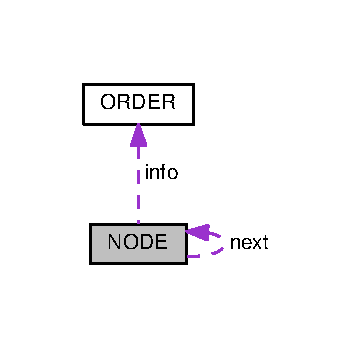
\includegraphics[width=169pt]{structNODE__coll__graph}
\end{center}
\end{figure}
\subsubsection*{Public Attributes}
\begin{DoxyCompactItemize}
\item 
\hyperlink{structORDER}{O\+R\+D\+E\+R} \hyperlink{structNODE_a8ae24fb8df6ea326ce23cab9331efdd6}{info}
\item 
\hyperlink{structNODE}{N\+O\+D\+E} $\ast$ \hyperlink{structNODE_a078472e8ab2d2fe38e052f5c2a425618}{next}
\end{DoxyCompactItemize}


\subsubsection{Detailed Description}
struct \hyperlink{structNODE}{N\+O\+D\+E} that will be used to make linked list 

\subsubsection{Member Data Documentation}
\hypertarget{structNODE_a8ae24fb8df6ea326ce23cab9331efdd6}{\index{N\+O\+D\+E@{N\+O\+D\+E}!info@{info}}
\index{info@{info}!N\+O\+D\+E@{N\+O\+D\+E}}
\paragraph[{info}]{\setlength{\rightskip}{0pt plus 5cm}{\bf O\+R\+D\+E\+R} N\+O\+D\+E\+::info}}\label{structNODE_a8ae24fb8df6ea326ce23cab9331efdd6}
\hypertarget{structNODE_a078472e8ab2d2fe38e052f5c2a425618}{\index{N\+O\+D\+E@{N\+O\+D\+E}!next@{next}}
\index{next@{next}!N\+O\+D\+E@{N\+O\+D\+E}}
\paragraph[{next}]{\setlength{\rightskip}{0pt plus 5cm}{\bf N\+O\+D\+E}$\ast$ N\+O\+D\+E\+::next}}\label{structNODE_a078472e8ab2d2fe38e052f5c2a425618}


The documentation for this struct was generated from the following file\+:\begin{DoxyCompactItemize}
\item 
\hyperlink{lab_8h}{lab.\+h}\end{DoxyCompactItemize}

\hypertarget{structORDER}{\subsection{O\+R\+D\+E\+R Struct Reference}
\label{structORDER}\index{O\+R\+D\+E\+R@{O\+R\+D\+E\+R}}
}


struct named \hyperlink{structORDER}{O\+R\+D\+E\+R} which will have the name of the pizza and the address for delivery  




{\ttfamily \#include $<$lab.\+h$>$}

\subsubsection*{Public Attributes}
\begin{DoxyCompactItemize}
\item 
std\+::string \hyperlink{structORDER_aea87cd05ef2f7d3f6b2c5b9eebd0199d}{info}
\item 
std\+::string \hyperlink{structORDER_a501ab180a46b15c372b77037ef5b3edc}{addr}
\end{DoxyCompactItemize}


\subsubsection{Detailed Description}
struct named \hyperlink{structORDER}{O\+R\+D\+E\+R} which will have the name of the pizza and the address for delivery 

\subsubsection{Member Data Documentation}
\hypertarget{structORDER_a501ab180a46b15c372b77037ef5b3edc}{\index{O\+R\+D\+E\+R@{O\+R\+D\+E\+R}!addr@{addr}}
\index{addr@{addr}!O\+R\+D\+E\+R@{O\+R\+D\+E\+R}}
\paragraph[{addr}]{\setlength{\rightskip}{0pt plus 5cm}std\+::string O\+R\+D\+E\+R\+::addr}}\label{structORDER_a501ab180a46b15c372b77037ef5b3edc}
\hypertarget{structORDER_aea87cd05ef2f7d3f6b2c5b9eebd0199d}{\index{O\+R\+D\+E\+R@{O\+R\+D\+E\+R}!info@{info}}
\index{info@{info}!O\+R\+D\+E\+R@{O\+R\+D\+E\+R}}
\paragraph[{info}]{\setlength{\rightskip}{0pt plus 5cm}std\+::string O\+R\+D\+E\+R\+::info}}\label{structORDER_aea87cd05ef2f7d3f6b2c5b9eebd0199d}


The documentation for this struct was generated from the following file\+:\begin{DoxyCompactItemize}
\item 
\hyperlink{lab_8h}{lab.\+h}\end{DoxyCompactItemize}

\hypertarget{classRBQUEUE}{\subsection{R\+B\+Q\+U\+E\+U\+E Class Reference}
\label{classRBQUEUE}\index{R\+B\+Q\+U\+E\+U\+E@{R\+B\+Q\+U\+E\+U\+E}}
}


{\ttfamily \#include $<$lab.\+h$>$}

\subsubsection*{Public Member Functions}
\begin{DoxyCompactItemize}
\item 
\hyperlink{classRBQUEUE_a7e58de52e8ee8cb73332477746cd4a99}{R\+B\+Q\+U\+E\+U\+E} ()
\begin{DoxyCompactList}\small\item\em constructor of the ring buffer queue which sets the private data members to 0 \end{DoxyCompactList}\item 
\hyperlink{classRBQUEUE_a4216cbcdbbf756fb92e2554923c8f9fc}{$\sim$\+R\+B\+Q\+U\+E\+U\+E} ()
\begin{DoxyCompactList}\small\item\em destructor of the ring buffer queue which deletes all the data in the queue \end{DoxyCompactList}\item 
bool \hyperlink{classRBQUEUE_a14a2d1391fe60a74ff7d8dd4cec7454e}{Insert} (std\+::string s)
\begin{DoxyCompactList}\small\item\em insert adds data into the queue \end{DoxyCompactList}\item 
bool \hyperlink{classRBQUEUE_a64ca2c69a4e8f81d5ed0fd5dc6faf443}{Remove} (std\+::string \&s)
\begin{DoxyCompactList}\small\item\em removed data from the queue \end{DoxyCompactList}\item 
bool \hyperlink{classRBQUEUE_a3a97717d7831d8489981beceafac4122}{is\+Empty} ()
\begin{DoxyCompactList}\small\item\em checks if the queue is empty \end{DoxyCompactList}\item 
bool \hyperlink{classRBQUEUE_ae8a4143bab8b1d41b0b3d2102ca2acbf}{is\+Full} ()
\begin{DoxyCompactList}\small\item\em checks if the queue is full \end{DoxyCompactList}\item 
std\+::string \hyperlink{classRBQUEUE_a07b611e131d8f1b51579c4f760bb60ad}{get\+R\+Qcontents} ()
\begin{DoxyCompactList}\small\item\em gives the user all the data that is present in the queue \end{DoxyCompactList}\end{DoxyCompactItemize}


\subsubsection{Constructor \& Destructor Documentation}
\hypertarget{classRBQUEUE_a7e58de52e8ee8cb73332477746cd4a99}{\index{R\+B\+Q\+U\+E\+U\+E@{R\+B\+Q\+U\+E\+U\+E}!R\+B\+Q\+U\+E\+U\+E@{R\+B\+Q\+U\+E\+U\+E}}
\index{R\+B\+Q\+U\+E\+U\+E@{R\+B\+Q\+U\+E\+U\+E}!R\+B\+Q\+U\+E\+U\+E@{R\+B\+Q\+U\+E\+U\+E}}
\paragraph[{R\+B\+Q\+U\+E\+U\+E}]{\setlength{\rightskip}{0pt plus 5cm}R\+B\+Q\+U\+E\+U\+E\+::\+R\+B\+Q\+U\+E\+U\+E (
\begin{DoxyParamCaption}
{}
\end{DoxyParamCaption}
)\hspace{0.3cm}{\ttfamily [inline]}}}\label{classRBQUEUE_a7e58de52e8ee8cb73332477746cd4a99}


constructor of the ring buffer queue which sets the private data members to 0 


\begin{DoxyCode}
139 \{front = rear = 0;\}
\end{DoxyCode}
\hypertarget{classRBQUEUE_a4216cbcdbbf756fb92e2554923c8f9fc}{\index{R\+B\+Q\+U\+E\+U\+E@{R\+B\+Q\+U\+E\+U\+E}!````~R\+B\+Q\+U\+E\+U\+E@{$\sim$\+R\+B\+Q\+U\+E\+U\+E}}
\index{````~R\+B\+Q\+U\+E\+U\+E@{$\sim$\+R\+B\+Q\+U\+E\+U\+E}!R\+B\+Q\+U\+E\+U\+E@{R\+B\+Q\+U\+E\+U\+E}}
\paragraph[{$\sim$\+R\+B\+Q\+U\+E\+U\+E}]{\setlength{\rightskip}{0pt plus 5cm}R\+B\+Q\+U\+E\+U\+E\+::$\sim$\+R\+B\+Q\+U\+E\+U\+E (
\begin{DoxyParamCaption}
{}
\end{DoxyParamCaption}
)\hspace{0.3cm}{\ttfamily [inline]}}}\label{classRBQUEUE_a4216cbcdbbf756fb92e2554923c8f9fc}


destructor of the ring buffer queue which deletes all the data in the queue 


\begin{DoxyCode}
143 \{\}
\end{DoxyCode}


\subsubsection{Member Function Documentation}
\hypertarget{classRBQUEUE_a07b611e131d8f1b51579c4f760bb60ad}{\index{R\+B\+Q\+U\+E\+U\+E@{R\+B\+Q\+U\+E\+U\+E}!get\+R\+Qcontents@{get\+R\+Qcontents}}
\index{get\+R\+Qcontents@{get\+R\+Qcontents}!R\+B\+Q\+U\+E\+U\+E@{R\+B\+Q\+U\+E\+U\+E}}
\paragraph[{get\+R\+Qcontents}]{\setlength{\rightskip}{0pt plus 5cm}std\+::string R\+B\+Q\+U\+E\+U\+E\+::get\+R\+Qcontents (
\begin{DoxyParamCaption}
{}
\end{DoxyParamCaption}
)}}\label{classRBQUEUE_a07b611e131d8f1b51579c4f760bb60ad}


gives the user all the data that is present in the queue 

\begin{DoxyReturn}{Returns}
string containing all the data that is stored in the queue 
\end{DoxyReturn}

\begin{DoxyCode}
4 \{
5     \textcolor{keywordtype}{int} curr;
6     std::string drivers;
7     \textcolor{keywordflow}{for}(\textcolor{keywordtype}{int} curr=front; curr<rear; curr=nextIndex(curr))\textcolor{comment}{//sets current to the front, if curr is less than
       rear, move current to the next index after front}
8     \{
9         drivers += buf[curr] + \textcolor{stringliteral}{"\(\backslash\)n"}; \textcolor{comment}{//stores all the data into the string}
10         
11         \}
12     \textcolor{keywordflow}{return} drivers; \textcolor{comment}{//returns the string with all the data}
13     \}
\end{DoxyCode}
\hypertarget{classRBQUEUE_a14a2d1391fe60a74ff7d8dd4cec7454e}{\index{R\+B\+Q\+U\+E\+U\+E@{R\+B\+Q\+U\+E\+U\+E}!Insert@{Insert}}
\index{Insert@{Insert}!R\+B\+Q\+U\+E\+U\+E@{R\+B\+Q\+U\+E\+U\+E}}
\paragraph[{Insert}]{\setlength{\rightskip}{0pt plus 5cm}bool R\+B\+Q\+U\+E\+U\+E\+::\+Insert (
\begin{DoxyParamCaption}
\item[{std\+::string}]{s}
\end{DoxyParamCaption}
)}}\label{classRBQUEUE_a14a2d1391fe60a74ff7d8dd4cec7454e}


insert adds data into the queue 


\begin{DoxyParams}[1]{Parameters}
\mbox{\tt in}  & {\em s} & is the data that will be added into the queue \\
\hline
\end{DoxyParams}
\begin{DoxyReturn}{Returns}
boolean indication if the data was inserted successfully 
\end{DoxyReturn}

\begin{DoxyCode}
4 \{
5     \textcolor{keywordflow}{if}(\hyperlink{classRBQUEUE_ae8a4143bab8b1d41b0b3d2102ca2acbf}{isFull}())\textcolor{comment}{// if the Q is full}
6     \{
7         \textcolor{keywordflow}{return} \textcolor{keyword}{false};
8         \}
9     buf[rear]= s; \textcolor{comment}{// inserts the data}
10     rear = nextIndex(rear); \textcolor{comment}{// rear is the next available index}
11     \textcolor{keywordflow}{return} \textcolor{keyword}{true};
12     \}
\end{DoxyCode}
\hypertarget{classRBQUEUE_a3a97717d7831d8489981beceafac4122}{\index{R\+B\+Q\+U\+E\+U\+E@{R\+B\+Q\+U\+E\+U\+E}!is\+Empty@{is\+Empty}}
\index{is\+Empty@{is\+Empty}!R\+B\+Q\+U\+E\+U\+E@{R\+B\+Q\+U\+E\+U\+E}}
\paragraph[{is\+Empty}]{\setlength{\rightskip}{0pt plus 5cm}bool R\+B\+Q\+U\+E\+U\+E\+::is\+Empty (
\begin{DoxyParamCaption}
{}
\end{DoxyParamCaption}
)\hspace{0.3cm}{\ttfamily [inline]}}}\label{classRBQUEUE_a3a97717d7831d8489981beceafac4122}


checks if the queue is empty 

\begin{DoxyReturn}{Returns}
boolean indication if the queue is empty or not 
\end{DoxyReturn}

\begin{DoxyCode}
160 \{\textcolor{keywordflow}{return} (front == rear);\}
\end{DoxyCode}
\hypertarget{classRBQUEUE_ae8a4143bab8b1d41b0b3d2102ca2acbf}{\index{R\+B\+Q\+U\+E\+U\+E@{R\+B\+Q\+U\+E\+U\+E}!is\+Full@{is\+Full}}
\index{is\+Full@{is\+Full}!R\+B\+Q\+U\+E\+U\+E@{R\+B\+Q\+U\+E\+U\+E}}
\paragraph[{is\+Full}]{\setlength{\rightskip}{0pt plus 5cm}bool R\+B\+Q\+U\+E\+U\+E\+::is\+Full (
\begin{DoxyParamCaption}
{}
\end{DoxyParamCaption}
)\hspace{0.3cm}{\ttfamily [inline]}}}\label{classRBQUEUE_ae8a4143bab8b1d41b0b3d2102ca2acbf}


checks if the queue is full 

\begin{DoxyReturn}{Returns}
boolean indication if the queue is full or not 
\end{DoxyReturn}

\begin{DoxyCode}
165 \{\textcolor{keywordflow}{return} (nextIndex(rear) == front);\}
\end{DoxyCode}
\hypertarget{classRBQUEUE_a64ca2c69a4e8f81d5ed0fd5dc6faf443}{\index{R\+B\+Q\+U\+E\+U\+E@{R\+B\+Q\+U\+E\+U\+E}!Remove@{Remove}}
\index{Remove@{Remove}!R\+B\+Q\+U\+E\+U\+E@{R\+B\+Q\+U\+E\+U\+E}}
\paragraph[{Remove}]{\setlength{\rightskip}{0pt plus 5cm}bool R\+B\+Q\+U\+E\+U\+E\+::\+Remove (
\begin{DoxyParamCaption}
\item[{std\+::string \&}]{s}
\end{DoxyParamCaption}
)}}\label{classRBQUEUE_a64ca2c69a4e8f81d5ed0fd5dc6faf443}


removed data from the queue 


\begin{DoxyParams}[1]{Parameters}
\mbox{\tt out}  & {\em s} & is the data that will be removed from the queue \\
\hline
\end{DoxyParams}
\begin{DoxyReturn}{Returns}
boolean indication if the data was removed successfully 
\end{DoxyReturn}

\begin{DoxyCode}
4 \{
5     \textcolor{keywordflow}{if}(\hyperlink{classRBQUEUE_a3a97717d7831d8489981beceafac4122}{isEmpty}())
6     \{
7         \textcolor{keywordflow}{return} \textcolor{keyword}{false};
8         \}
9    s = buf[front]; \textcolor{comment}{//sets s to the value being removed}
10     front = nextIndex(front); \textcolor{comment}{// moves front to the next index}
11     \textcolor{keywordflow}{return} \textcolor{keyword}{true};
12     \}
\end{DoxyCode}


The documentation for this class was generated from the following files\+:\begin{DoxyCompactItemize}
\item 
\hyperlink{lab_8h}{lab.\+h}\item 
\hyperlink{getRQcontents_8cpp}{get\+R\+Qcontents.\+cpp}\item 
\hyperlink{insert_8cpp}{insert.\+cpp}\item 
\hyperlink{remove_8cpp}{remove.\+cpp}\end{DoxyCompactItemize}

\section{File Documentation}
\hypertarget{addBackDr__cb_8cpp}{\subsection{add\+Back\+Dr\+\_\+cb.\+cpp File Reference}
\label{addBackDr__cb_8cpp}\index{add\+Back\+Dr\+\_\+cb.\+cpp@{add\+Back\+Dr\+\_\+cb.\+cpp}}
}
{\ttfamily \#include \char`\"{}lab.\+h\char`\"{}}\\*
Include dependency graph for add\+Back\+Dr\+\_\+cb.\+cpp\+:\nopagebreak
\begin{figure}[H]
\begin{center}
\leavevmode
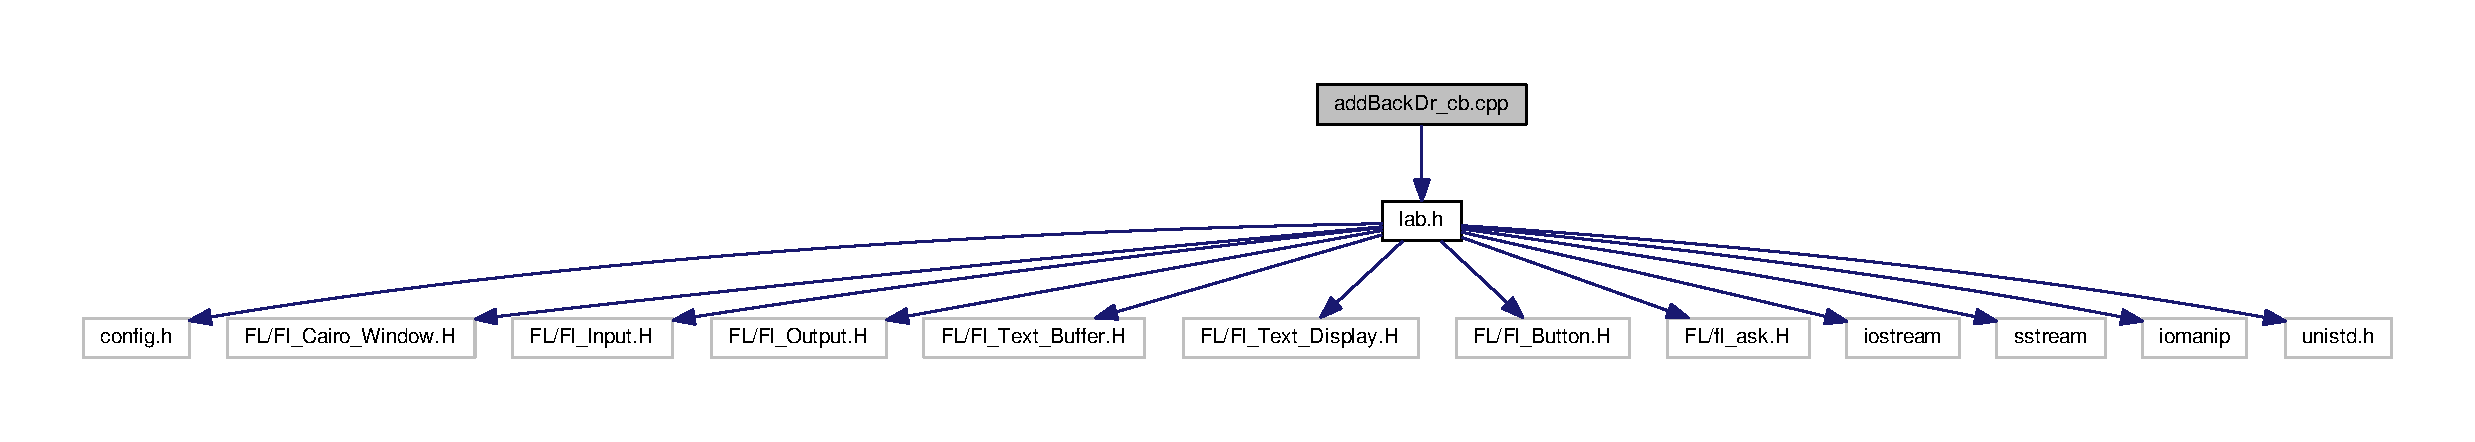
\includegraphics[width=350pt]{addBackDr__cb_8cpp__incl}
\end{center}
\end{figure}
\subsubsection*{Functions}
\begin{DoxyCompactItemize}
\item 
void \hyperlink{addBackDr__cb_8cpp_a8cfdf48b45c7a996149651583c14266d}{add\+Back\+Dr\+\_\+cb} (void $\ast$)
\begin{DoxyCompactList}\small\item\em This is the callback function called fron delivery which adds the driver back in the queue after they deliver the pizza void pointers not used return void. \end{DoxyCompactList}\end{DoxyCompactItemize}


\subsubsection{Function Documentation}
\hypertarget{addBackDr__cb_8cpp_a8cfdf48b45c7a996149651583c14266d}{\index{add\+Back\+Dr\+\_\+cb.\+cpp@{add\+Back\+Dr\+\_\+cb.\+cpp}!add\+Back\+Dr\+\_\+cb@{add\+Back\+Dr\+\_\+cb}}
\index{add\+Back\+Dr\+\_\+cb@{add\+Back\+Dr\+\_\+cb}!add\+Back\+Dr\+\_\+cb.\+cpp@{add\+Back\+Dr\+\_\+cb.\+cpp}}
\paragraph[{add\+Back\+Dr\+\_\+cb}]{\setlength{\rightskip}{0pt plus 5cm}void add\+Back\+Dr\+\_\+cb (
\begin{DoxyParamCaption}
\item[{void $\ast$}]{}
\end{DoxyParamCaption}
)}}\label{addBackDr__cb_8cpp_a8cfdf48b45c7a996149651583c14266d}


This is the callback function called fron delivery which adds the driver back in the queue after they deliver the pizza void pointers not used return void. 


\begin{DoxyCode}
4 \{
5     std::string Dback; \textcolor{comment}{//will be used to display alert}
6     \hyperlink{lab_8h_a0fc2dbd38da95932f1a2331561cf9a4e}{currD}.\hyperlink{classRBQUEUE_a64ca2c69a4e8f81d5ed0fd5dc6faf443}{Remove}(Dback);\textcolor{comment}{//removes the driver from the queue of drivers who are currently
       delivering}
7     \hyperlink{lab_8h_a87b7985f8561b2ac6c65961ab55b326e}{d}.\hyperlink{classRBQUEUE_a14a2d1391fe60a74ff7d8dd4cec7454e}{Insert}(Dback); \textcolor{comment}{//inserts the driver to the original driver queue who is ready to deliver}
8     \hyperlink{lab_8h_a5d487f4a7b5d36f823b8b1cb3db75aa4}{dbuff}->text((\hyperlink{lab_8h_a87b7985f8561b2ac6c65961ab55b326e}{d}.\hyperlink{classRBQUEUE_a07b611e131d8f1b51579c4f760bb60ad}{getRQcontents}().c\_str())); \textcolor{comment}{//updates the text in FLTK}
9     std::string alrt; \textcolor{comment}{//string that will help display alert}
10     alrt = Dback + \textcolor{stringliteral}{" is back from delivery"};
11     fl\_alert(alrt.c\_str()); \textcolor{comment}{//shows alert when the driver is back}
12     \}
\end{DoxyCode}

\hypertarget{cook__cb_8cpp}{\subsection{cook\+\_\+cb.\+cpp File Reference}
\label{cook__cb_8cpp}\index{cook\+\_\+cb.\+cpp@{cook\+\_\+cb.\+cpp}}
}
{\ttfamily \#include \char`\"{}lab.\+h\char`\"{}}\\*
Include dependency graph for cook\+\_\+cb.\+cpp\+:\nopagebreak
\begin{figure}[H]
\begin{center}
\leavevmode
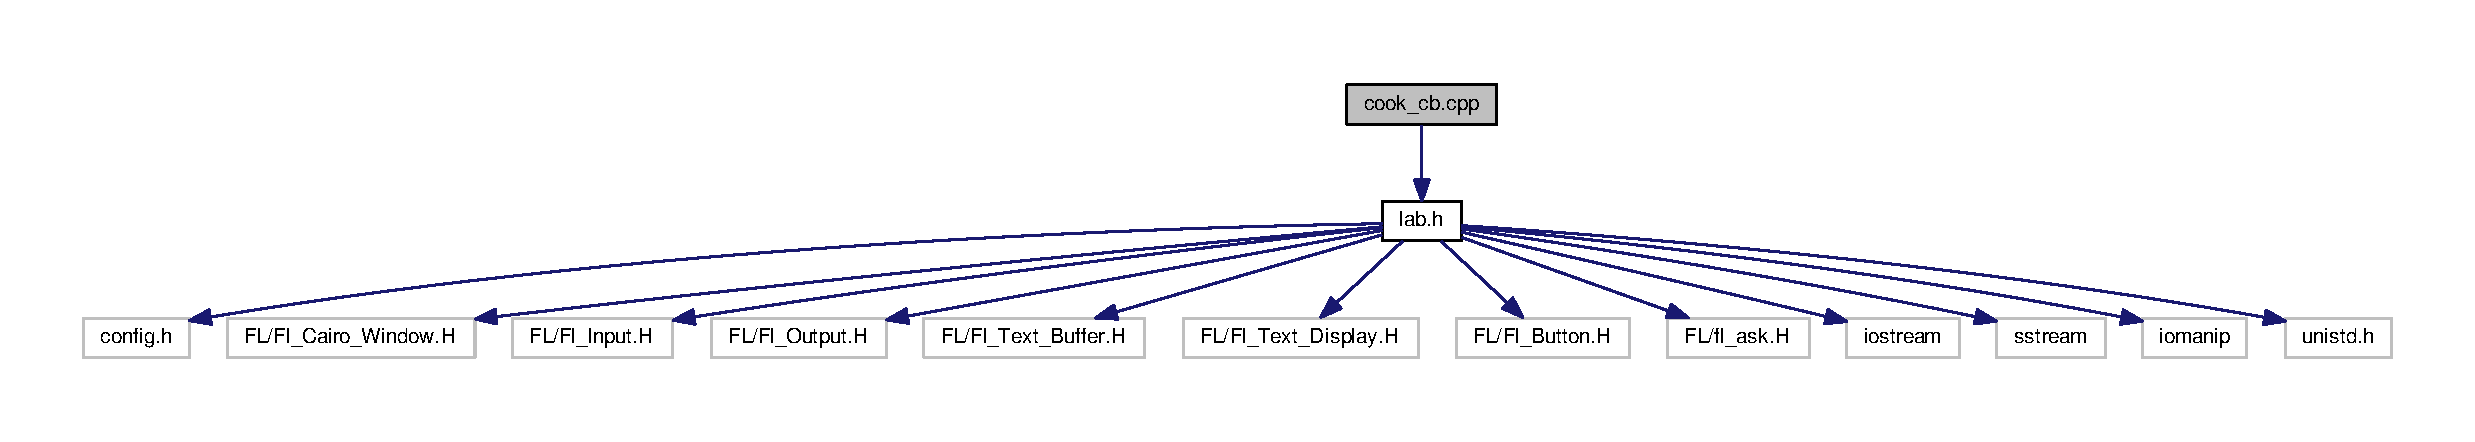
\includegraphics[width=350pt]{cook__cb_8cpp__incl}
\end{center}
\end{figure}
\subsubsection*{Functions}
\begin{DoxyCompactItemize}
\item 
void \hyperlink{cook__cb_8cpp_abb6fd11336b6e04e134b70abc225a8f6}{cook\+\_\+cb} (void $\ast$)
\begin{DoxyCompactList}\small\item\em This is the callback function called from the order\+\_\+cb function which cooks the pizza void pointer not used return void. \end{DoxyCompactList}\end{DoxyCompactItemize}


\subsubsection{Function Documentation}
\hypertarget{cook__cb_8cpp_abb6fd11336b6e04e134b70abc225a8f6}{\index{cook\+\_\+cb.\+cpp@{cook\+\_\+cb.\+cpp}!cook\+\_\+cb@{cook\+\_\+cb}}
\index{cook\+\_\+cb@{cook\+\_\+cb}!cook\+\_\+cb.\+cpp@{cook\+\_\+cb.\+cpp}}
\paragraph[{cook\+\_\+cb}]{\setlength{\rightskip}{0pt plus 5cm}void cook\+\_\+cb (
\begin{DoxyParamCaption}
\item[{void $\ast$}]{}
\end{DoxyParamCaption}
)}}\label{cook__cb_8cpp_abb6fd11336b6e04e134b70abc225a8f6}


This is the callback function called from the order\+\_\+cb function which cooks the pizza void pointer not used return void. 


\begin{DoxyCode}
3 \{   
4     \hyperlink{lab_8h_a6131f0484df536b2c26a825ec37671a2}{o}.\hyperlink{classLLQUEUE_ab8d52943d24188adf0855a0ee9fa0afe}{Remove}(\hyperlink{lab_8h_a332f3283fc67e4d87244860ec1f0e880}{ord}); \textcolor{comment}{//removes the data from the order queue}
5     \hyperlink{lab_8h_aea2b8efadc87a819fe57c311d668e504}{buff}->text((\hyperlink{lab_8h_a6131f0484df536b2c26a825ec37671a2}{o}.\hyperlink{classLLQUEUE_a0e9bffdcd903a132b8f7899ccdbc0315}{getQcontent}().c\_str()));\textcolor{comment}{//updates the data for FLTK in the order Q}
6     \hyperlink{lab_8h_a5574ed76bfb4e719e874d19f2d247625}{c}.\hyperlink{classLLQUEUE_a2d53817739f7c273a3c0f14f7804c065}{Insert}(\hyperlink{lab_8h_a332f3283fc67e4d87244860ec1f0e880}{ord}); \textcolor{comment}{//inserts the data into the cooked Q}
7     
8     \hyperlink{lab_8h_a3a16cd8310a89f45962eb39b72bb9bb1}{cbuff}->text((\hyperlink{lab_8h_a5574ed76bfb4e719e874d19f2d247625}{c}.\hyperlink{classLLQUEUE_a0e9bffdcd903a132b8f7899ccdbc0315}{getQcontent}().c\_str())); \textcolor{comment}{//Updates the FLTK text box for cooked Q}
9     
10     std::string alrt = \hyperlink{lab_8h_a332f3283fc67e4d87244860ec1f0e880}{ord}.\hyperlink{structORDER_aea87cd05ef2f7d3f6b2c5b9eebd0199d}{info} + \textcolor{stringliteral}{" is cooked"};
11     fl\_alert(alrt.c\_str()); \textcolor{comment}{//shows alert that the pizza is cooked}
12     
13     Fl::add\_timeout(3,\hyperlink{delivery__cb_8cpp_a991653c5063a84cb2fa299a9738892da}{delivery\_cb}); \textcolor{comment}{//calls back the delivery\_cb function with 3 sec delay for
       us to actually see whats happening}
14     
15 \}
\end{DoxyCode}

\hypertarget{delivery__cb_8cpp}{\subsection{delivery\+\_\+cb.\+cpp File Reference}
\label{delivery__cb_8cpp}\index{delivery\+\_\+cb.\+cpp@{delivery\+\_\+cb.\+cpp}}
}
{\ttfamily \#include \char`\"{}lab.\+h\char`\"{}}\\*
Include dependency graph for delivery\+\_\+cb.\+cpp\+:\nopagebreak
\begin{figure}[H]
\begin{center}
\leavevmode
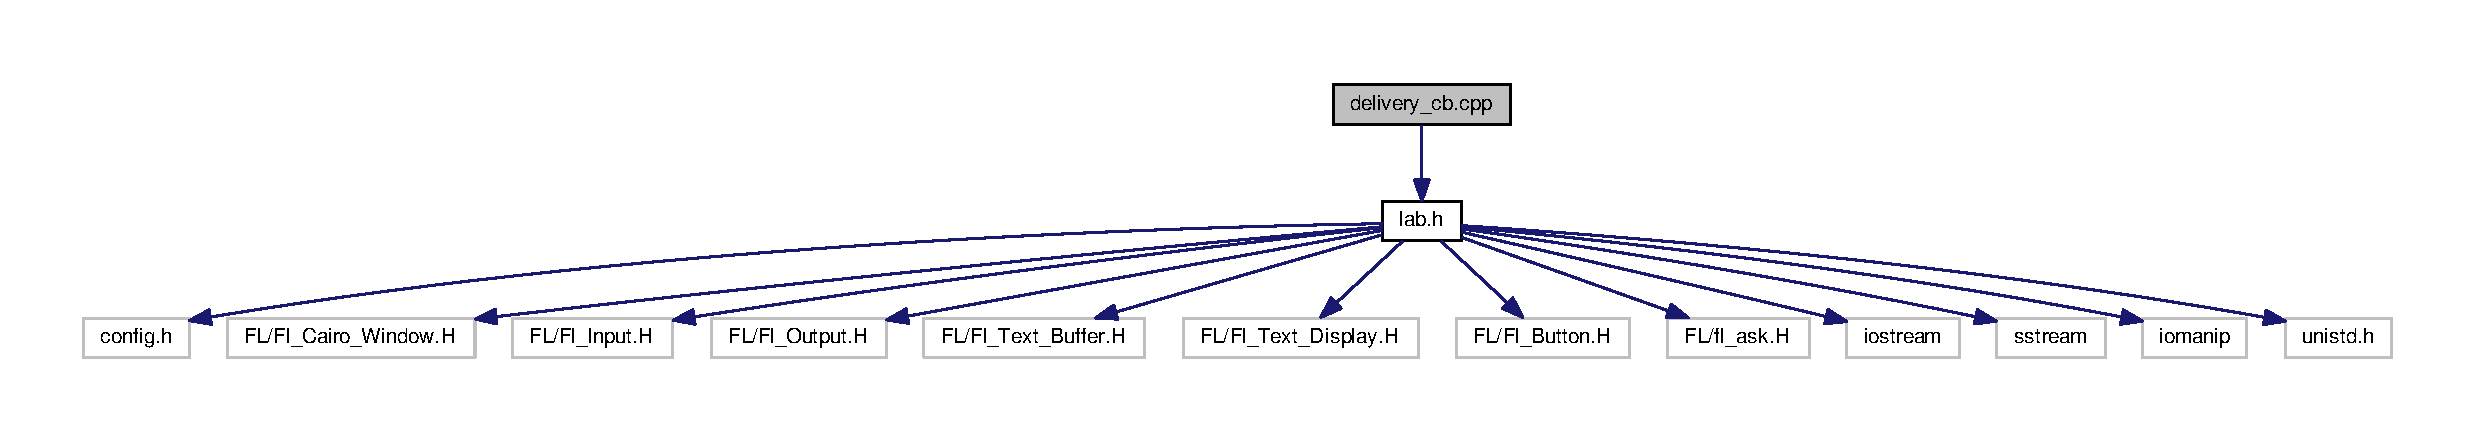
\includegraphics[width=350pt]{delivery__cb_8cpp__incl}
\end{center}
\end{figure}
\subsubsection*{Functions}
\begin{DoxyCompactItemize}
\item 
void \hyperlink{delivery__cb_8cpp_a991653c5063a84cb2fa299a9738892da}{delivery\+\_\+cb} (void $\ast$)
\begin{DoxyCompactList}\small\item\em This is the callback function called from the cook\+\_\+cb function which assigns and send drivers out for delivery after the pizza is cooked void pointers not used return void. \end{DoxyCompactList}\end{DoxyCompactItemize}


\subsubsection{Function Documentation}
\hypertarget{delivery__cb_8cpp_a991653c5063a84cb2fa299a9738892da}{\index{delivery\+\_\+cb.\+cpp@{delivery\+\_\+cb.\+cpp}!delivery\+\_\+cb@{delivery\+\_\+cb}}
\index{delivery\+\_\+cb@{delivery\+\_\+cb}!delivery\+\_\+cb.\+cpp@{delivery\+\_\+cb.\+cpp}}
\paragraph[{delivery\+\_\+cb}]{\setlength{\rightskip}{0pt plus 5cm}void delivery\+\_\+cb (
\begin{DoxyParamCaption}
\item[{void $\ast$}]{}
\end{DoxyParamCaption}
)}}\label{delivery__cb_8cpp_a991653c5063a84cb2fa299a9738892da}


This is the callback function called from the cook\+\_\+cb function which assigns and send drivers out for delivery after the pizza is cooked void pointers not used return void. 


\begin{DoxyCode}
4 \{   
5     
6      \textcolor{keywordflow}{if}(\hyperlink{lab_8h_a87b7985f8561b2ac6c65961ab55b326e}{d}.\hyperlink{classRBQUEUE_a3a97717d7831d8489981beceafac4122}{isEmpty}()) \textcolor{comment}{//checks if the drivers Q is empty}
7     \{
8        fl\_alert(\textcolor{stringliteral}{"Not enough drivers"}); \textcolor{comment}{//shows alerts that there are no more drivers}
9        Fl::add\_timeout(5,\hyperlink{delivery__cb_8cpp_a991653c5063a84cb2fa299a9738892da}{delivery\_cb}); \textcolor{comment}{//checks again if there are any drivers in the Q after 5
       sec}
10         \}
11     \textcolor{keywordflow}{else}
12     \{
13         std::string dname;
14         \hyperlink{lab_8h_a87b7985f8561b2ac6c65961ab55b326e}{d}.\hyperlink{classRBQUEUE_a64ca2c69a4e8f81d5ed0fd5dc6faf443}{Remove}(dname);\textcolor{comment}{//removes the driver who is ready for delivery}
15         \hyperlink{lab_8h_a0fc2dbd38da95932f1a2331561cf9a4e}{currD}.\hyperlink{classRBQUEUE_a14a2d1391fe60a74ff7d8dd4cec7454e}{Insert}(dname); \textcolor{comment}{//puts the same driver in a different RBQ which is for the drivers
       who are out for delivery}
16         \hyperlink{lab_8h_a5574ed76bfb4e719e874d19f2d247625}{c}.\hyperlink{classLLQUEUE_ab8d52943d24188adf0855a0ee9fa0afe}{Remove}(\hyperlink{lab_8h_a332f3283fc67e4d87244860ec1f0e880}{ord});\textcolor{comment}{//removes the pizza from the cooked Q}
17         std::string temp = dname + \textcolor{stringliteral}{" is delivering the "}+ \hyperlink{lab_8h_a332f3283fc67e4d87244860ec1f0e880}{ord}.\hyperlink{structORDER_aea87cd05ef2f7d3f6b2c5b9eebd0199d}{info} + \textcolor{stringliteral}{" to "} + 
      \hyperlink{lab_8h_a332f3283fc67e4d87244860ec1f0e880}{ord}.\hyperlink{structORDER_a501ab180a46b15c372b77037ef5b3edc}{addr};
18         fl\_alert(temp.c\_str());\textcolor{comment}{//alert that shows who is delivering the pizaa and where}
19         \hyperlink{lab_8h_a3a16cd8310a89f45962eb39b72bb9bb1}{cbuff}->text((\hyperlink{lab_8h_a5574ed76bfb4e719e874d19f2d247625}{c}.\hyperlink{classLLQUEUE_a0e9bffdcd903a132b8f7899ccdbc0315}{getQcontent}().c\_str())); \textcolor{comment}{// updates FLTK text in cooked Q box}
20         \hyperlink{lab_8h_a5d487f4a7b5d36f823b8b1cb3db75aa4}{dbuff}->text((\hyperlink{lab_8h_a87b7985f8561b2ac6c65961ab55b326e}{d}.\hyperlink{classRBQUEUE_a07b611e131d8f1b51579c4f760bb60ad}{getRQcontents}().c\_str())); \textcolor{comment}{// updates FLTK text in drivers Q box}
21         Fl::add\_timeout(100,\hyperlink{addBackDr__cb_8cpp_a8cfdf48b45c7a996149651583c14266d}{addBackDr\_cb}); \textcolor{comment}{//cb to the function which adds the drivers back
       after they do delivery}
22         \}
23    
24     \}
\end{DoxyCode}

\hypertarget{driver__cb_8cpp}{\subsection{driver\+\_\+cb.\+cpp File Reference}
\label{driver__cb_8cpp}\index{driver\+\_\+cb.\+cpp@{driver\+\_\+cb.\+cpp}}
}
{\ttfamily \#include \char`\"{}lab.\+h\char`\"{}}\\*
Include dependency graph for driver\+\_\+cb.\+cpp\+:\nopagebreak
\begin{figure}[H]
\begin{center}
\leavevmode
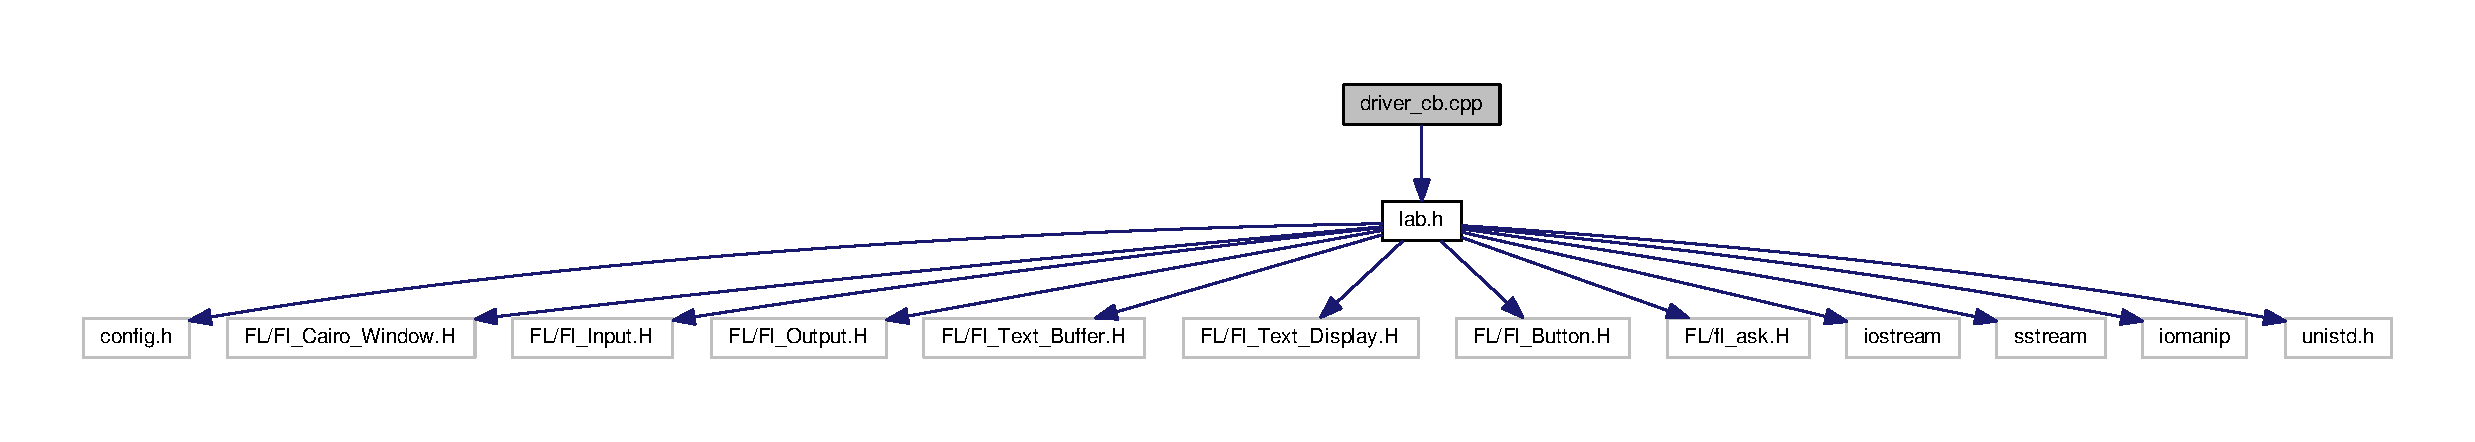
\includegraphics[width=350pt]{driver__cb_8cpp__incl}
\end{center}
\end{figure}
\subsubsection*{Functions}
\begin{DoxyCompactItemize}
\item 
void \hyperlink{driver__cb_8cpp_a2edcbf888225d725652a44b6a98d64c2}{driver\+\_\+cb} (void $\ast$)
\begin{DoxyCompactList}\small\item\em This is the callback function to add drivers manually void pointers not used return void. \end{DoxyCompactList}\end{DoxyCompactItemize}


\subsubsection{Function Documentation}
\hypertarget{driver__cb_8cpp_a2edcbf888225d725652a44b6a98d64c2}{\index{driver\+\_\+cb.\+cpp@{driver\+\_\+cb.\+cpp}!driver\+\_\+cb@{driver\+\_\+cb}}
\index{driver\+\_\+cb@{driver\+\_\+cb}!driver\+\_\+cb.\+cpp@{driver\+\_\+cb.\+cpp}}
\paragraph[{driver\+\_\+cb}]{\setlength{\rightskip}{0pt plus 5cm}void driver\+\_\+cb (
\begin{DoxyParamCaption}
\item[{void $\ast$}]{}
\end{DoxyParamCaption}
)}}\label{driver__cb_8cpp_a2edcbf888225d725652a44b6a98d64c2}


This is the callback function to add drivers manually void pointers not used return void. 


\begin{DoxyCode}
4 \{   
5    fl\_alert(\hyperlink{lab_8h_a6f3dbb90a24ffb00549fdd15a79cbd66}{driver}->value()); \textcolor{comment}{//shows alert for the driver who is being added by the user}
6    std::string name;
7    name = \hyperlink{lab_8h_a6f3dbb90a24ffb00549fdd15a79cbd66}{driver}->value();
8      \hyperlink{lab_8h_a87b7985f8561b2ac6c65961ab55b326e}{d}.\hyperlink{classRBQUEUE_a14a2d1391fe60a74ff7d8dd4cec7454e}{Insert}(name); \textcolor{comment}{//inserts the driver in the driversQ}
9     \hyperlink{lab_8h_a5d487f4a7b5d36f823b8b1cb3db75aa4}{dbuff}->text((\hyperlink{lab_8h_a87b7985f8561b2ac6c65961ab55b326e}{d}.\hyperlink{classRBQUEUE_a07b611e131d8f1b51579c4f760bb60ad}{getRQcontents}().c\_str())); \textcolor{comment}{// updates the FLTK driversQ box}
10     \}
\end{DoxyCode}

\hypertarget{getQcontent_8cpp}{\subsection{get\+Qcontent.\+cpp File Reference}
\label{getQcontent_8cpp}\index{get\+Qcontent.\+cpp@{get\+Qcontent.\+cpp}}
}
{\ttfamily \#include \char`\"{}lab.\+h\char`\"{}}\\*
Include dependency graph for get\+Qcontent.\+cpp\+:\nopagebreak
\begin{figure}[H]
\begin{center}
\leavevmode
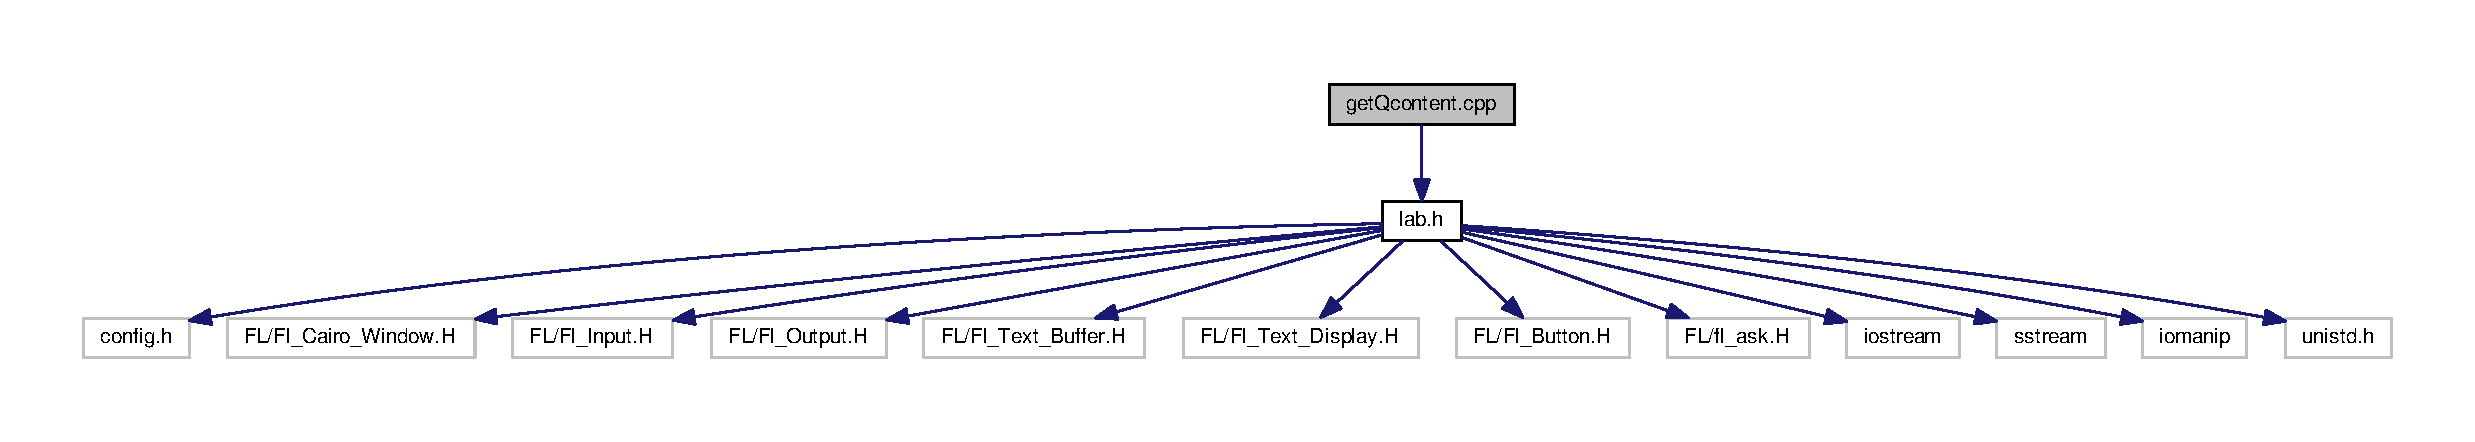
\includegraphics[width=350pt]{getQcontent_8cpp__incl}
\end{center}
\end{figure}

\hypertarget{getRQcontents_8cpp}{\subsection{get\+R\+Qcontents.\+cpp File Reference}
\label{getRQcontents_8cpp}\index{get\+R\+Qcontents.\+cpp@{get\+R\+Qcontents.\+cpp}}
}
{\ttfamily \#include \char`\"{}lab.\+h\char`\"{}}\\*
Include dependency graph for get\+R\+Qcontents.\+cpp\+:\nopagebreak
\begin{figure}[H]
\begin{center}
\leavevmode
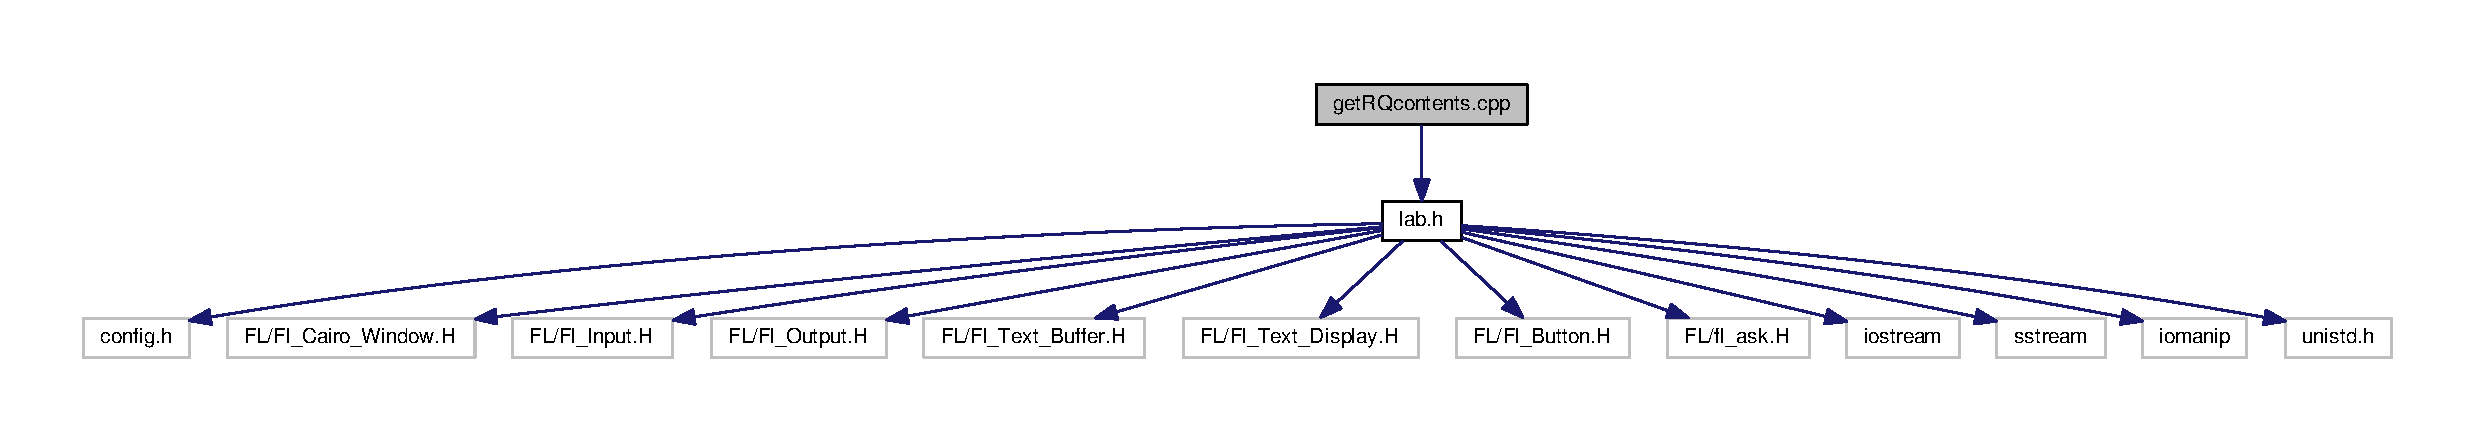
\includegraphics[width=350pt]{getRQcontents_8cpp__incl}
\end{center}
\end{figure}

\hypertarget{Insert_8cpp}{\subsection{Insert.\+cpp File Reference}
\label{Insert_8cpp}\index{Insert.\+cpp@{Insert.\+cpp}}
}
{\ttfamily \#include \char`\"{}lab.\+h\char`\"{}}\\*
Include dependency graph for Insert.\+cpp\+:\nopagebreak
\begin{figure}[H]
\begin{center}
\leavevmode
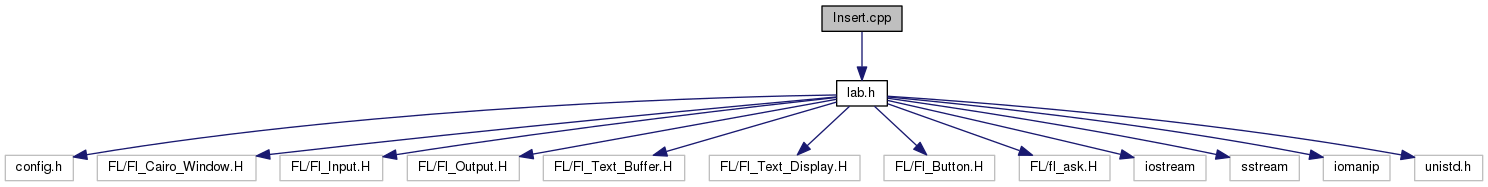
\includegraphics[width=350pt]{Insert_8cpp__incl}
\end{center}
\end{figure}

\input{insert_8cpp}
\hypertarget{lab_8dox}{\subsection{lab.\+dox File Reference}
\label{lab_8dox}\index{lab.\+dox@{lab.\+dox}}
}

\hypertarget{lab_8h}{\subsection{lab.\+h File Reference}
\label{lab_8h}\index{lab.\+h@{lab.\+h}}
}
{\ttfamily \#include \char`\"{}config.\+h\char`\"{}}\\*
{\ttfamily \#include $<$F\+L/\+Fl\+\_\+\+Cairo\+\_\+\+Window.\+H$>$}\\*
{\ttfamily \#include $<$F\+L/\+Fl\+\_\+\+Input.\+H$>$}\\*
{\ttfamily \#include $<$F\+L/\+Fl\+\_\+\+Output.\+H$>$}\\*
{\ttfamily \#include $<$F\+L/\+Fl\+\_\+\+Text\+\_\+\+Buffer.\+H$>$}\\*
{\ttfamily \#include $<$F\+L/\+Fl\+\_\+\+Text\+\_\+\+Display.\+H$>$}\\*
{\ttfamily \#include $<$F\+L/\+Fl\+\_\+\+Button.\+H$>$}\\*
{\ttfamily \#include $<$F\+L/fl\+\_\+ask.\+H$>$}\\*
{\ttfamily \#include $<$iostream$>$}\\*
{\ttfamily \#include $<$sstream$>$}\\*
{\ttfamily \#include $<$iomanip$>$}\\*
{\ttfamily \#include $<$unistd.\+h$>$}\\*
Include dependency graph for lab.\+h\+:\nopagebreak
\begin{figure}[H]
\begin{center}
\leavevmode
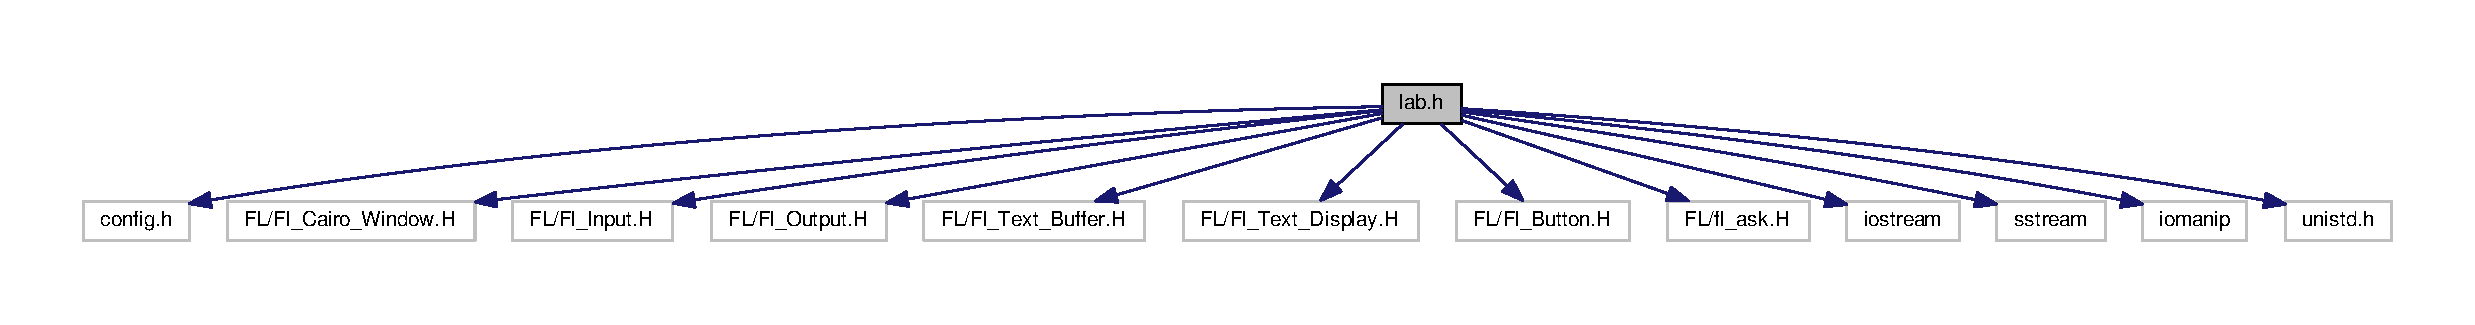
\includegraphics[width=350pt]{lab_8h__incl}
\end{center}
\end{figure}
This graph shows which files directly or indirectly include this file\+:\nopagebreak
\begin{figure}[H]
\begin{center}
\leavevmode
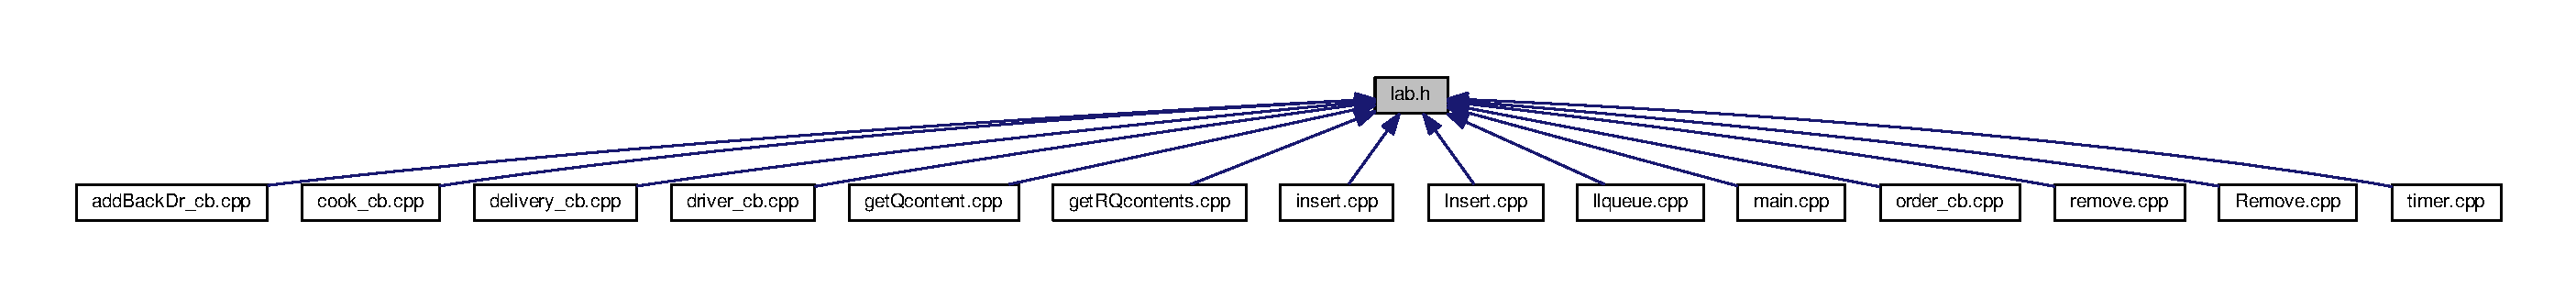
\includegraphics[width=350pt]{lab_8h__dep__incl}
\end{center}
\end{figure}
\subsubsection*{Classes}
\begin{DoxyCompactItemize}
\item 
struct \hyperlink{structORDER}{O\+R\+D\+E\+R}
\begin{DoxyCompactList}\small\item\em struct named \hyperlink{structORDER}{O\+R\+D\+E\+R} which will have the name of the pizza and the address for delivery \end{DoxyCompactList}\item 
struct \hyperlink{structNODE}{N\+O\+D\+E}
\begin{DoxyCompactList}\small\item\em struct \hyperlink{structNODE}{N\+O\+D\+E} that will be used to make linked list \end{DoxyCompactList}\item 
class \hyperlink{classLLQUEUE}{L\+L\+Q\+U\+E\+U\+E}
\item 
class \hyperlink{classRBQUEUE}{R\+B\+Q\+U\+E\+U\+E}
\end{DoxyCompactItemize}
\subsubsection*{Functions}
\begin{DoxyCompactItemize}
\item 
void \hyperlink{lab_8h_a547f84331a8c529348e1130ca169c69c}{order\+\_\+cb} (void $\ast$, void $\ast$)
\begin{DoxyCompactList}\small\item\em This is the callback function to order a pizza void pointers not used return void. \end{DoxyCompactList}\item 
void \hyperlink{lab_8h_a2edcbf888225d725652a44b6a98d64c2}{driver\+\_\+cb} (void $\ast$)
\begin{DoxyCompactList}\small\item\em This is the callback function to add drivers manually void pointers not used return void. \end{DoxyCompactList}\item 
void \hyperlink{lab_8h_abb6fd11336b6e04e134b70abc225a8f6}{cook\+\_\+cb} (void $\ast$)
\begin{DoxyCompactList}\small\item\em This is the callback function called from the order\+\_\+cb function which cooks the pizza void pointer not used return void. \end{DoxyCompactList}\item 
void \hyperlink{lab_8h_a991653c5063a84cb2fa299a9738892da}{delivery\+\_\+cb} (void $\ast$)
\begin{DoxyCompactList}\small\item\em This is the callback function called from the cook\+\_\+cb function which assigns and send drivers out for delivery after the pizza is cooked void pointers not used return void. \end{DoxyCompactList}\item 
void \hyperlink{lab_8h_a8cfdf48b45c7a996149651583c14266d}{add\+Back\+Dr\+\_\+cb} (void $\ast$)
\begin{DoxyCompactList}\small\item\em This is the callback function called fron delivery which adds the driver back in the queue after they deliver the pizza void pointers not used return void. \end{DoxyCompactList}\item 
void \hyperlink{lab_8h_a13ed8751dfa95731ad8930762493b16b}{timer} (void $\ast$)
\begin{DoxyCompactList}\small\item\em This is a time function which keeps track of the time void pointers not used return void. \end{DoxyCompactList}\end{DoxyCompactItemize}
\subsubsection*{Variables}
\begin{DoxyCompactItemize}
\item 
Fl\+\_\+\+Input $\ast$ \hyperlink{lab_8h_abf805c82a90897837d1c26ef915f1cd6}{pizza}
\item 
Fl\+\_\+\+Input $\ast$ \hyperlink{lab_8h_a0ce7586472726848924b4964b80e69ba}{address}
\item 
Fl\+\_\+\+Input $\ast$ \hyperlink{lab_8h_a6f3dbb90a24ffb00549fdd15a79cbd66}{driver}
\item 
Fl\+\_\+\+Output $\ast$ \hyperlink{lab_8h_a05c7f6e86cca5f4d0ebf44d1f5042c37}{watch}
\item 
Fl\+\_\+\+Text\+\_\+\+Buffer $\ast$ \hyperlink{lab_8h_aea2b8efadc87a819fe57c311d668e504}{buff}
\item 
Fl\+\_\+\+Text\+\_\+\+Buffer $\ast$ \hyperlink{lab_8h_a3a16cd8310a89f45962eb39b72bb9bb1}{cbuff}
\item 
Fl\+\_\+\+Text\+\_\+\+Buffer $\ast$ \hyperlink{lab_8h_a5d487f4a7b5d36f823b8b1cb3db75aa4}{dbuff}
\item 
Fl\+\_\+\+Text\+\_\+\+Display $\ast$ \hyperlink{lab_8h_a20a356461cec27fe0d294f923f7ebd01}{driver\+Q}
\item 
Fl\+\_\+\+Text\+\_\+\+Display $\ast$ \hyperlink{lab_8h_a23f917547a833922fd6bc8797cc04ee1}{order\+Q}
\item 
Fl\+\_\+\+Text\+\_\+\+Display $\ast$ \hyperlink{lab_8h_ad042fec17c471064617911f13dca15a8}{cooked\+Q}
\item 
const int \hyperlink{lab_8h_ad69f678058ac1e2c6d82212fd735b7a4}{B\+U\+F\+S\+I\+Z\+E} = 256
\item 
\hyperlink{structORDER}{O\+R\+D\+E\+R} \hyperlink{lab_8h_a332f3283fc67e4d87244860ec1f0e880}{ord}
\item 
\hyperlink{classLLQUEUE}{L\+L\+Q\+U\+E\+U\+E} \hyperlink{lab_8h_a6131f0484df536b2c26a825ec37671a2}{o}
\item 
\hyperlink{classLLQUEUE}{L\+L\+Q\+U\+E\+U\+E} \hyperlink{lab_8h_a5574ed76bfb4e719e874d19f2d247625}{c}
\item 
\hyperlink{classRBQUEUE}{R\+B\+Q\+U\+E\+U\+E} \hyperlink{lab_8h_a87b7985f8561b2ac6c65961ab55b326e}{d}
\item 
\hyperlink{classRBQUEUE}{R\+B\+Q\+U\+E\+U\+E} \hyperlink{lab_8h_a0fc2dbd38da95932f1a2331561cf9a4e}{curr\+D}
\end{DoxyCompactItemize}


\subsubsection{Function Documentation}
\hypertarget{lab_8h_a8cfdf48b45c7a996149651583c14266d}{\index{lab.\+h@{lab.\+h}!add\+Back\+Dr\+\_\+cb@{add\+Back\+Dr\+\_\+cb}}
\index{add\+Back\+Dr\+\_\+cb@{add\+Back\+Dr\+\_\+cb}!lab.\+h@{lab.\+h}}
\paragraph[{add\+Back\+Dr\+\_\+cb}]{\setlength{\rightskip}{0pt plus 5cm}void add\+Back\+Dr\+\_\+cb (
\begin{DoxyParamCaption}
\item[{void $\ast$}]{}
\end{DoxyParamCaption}
)}}\label{lab_8h_a8cfdf48b45c7a996149651583c14266d}


This is the callback function called fron delivery which adds the driver back in the queue after they deliver the pizza void pointers not used return void. 


\begin{DoxyCode}
4 \{
5     std::string Dback; \textcolor{comment}{//will be used to display alert}
6     \hyperlink{lab_8h_a0fc2dbd38da95932f1a2331561cf9a4e}{currD}.\hyperlink{classRBQUEUE_a64ca2c69a4e8f81d5ed0fd5dc6faf443}{Remove}(Dback);\textcolor{comment}{//removes the driver from the queue of drivers who are currently
       delivering}
7     \hyperlink{lab_8h_a87b7985f8561b2ac6c65961ab55b326e}{d}.\hyperlink{classRBQUEUE_a14a2d1391fe60a74ff7d8dd4cec7454e}{Insert}(Dback); \textcolor{comment}{//inserts the driver to the original driver queue who is ready to deliver}
8     \hyperlink{lab_8h_a5d487f4a7b5d36f823b8b1cb3db75aa4}{dbuff}->text((\hyperlink{lab_8h_a87b7985f8561b2ac6c65961ab55b326e}{d}.\hyperlink{classRBQUEUE_a07b611e131d8f1b51579c4f760bb60ad}{getRQcontents}().c\_str())); \textcolor{comment}{//updates the text in FLTK}
9     std::string alrt; \textcolor{comment}{//string that will help display alert}
10     alrt = Dback + \textcolor{stringliteral}{" is back from delivery"};
11     fl\_alert(alrt.c\_str()); \textcolor{comment}{//shows alert when the driver is back}
12     \}
\end{DoxyCode}
\hypertarget{lab_8h_abb6fd11336b6e04e134b70abc225a8f6}{\index{lab.\+h@{lab.\+h}!cook\+\_\+cb@{cook\+\_\+cb}}
\index{cook\+\_\+cb@{cook\+\_\+cb}!lab.\+h@{lab.\+h}}
\paragraph[{cook\+\_\+cb}]{\setlength{\rightskip}{0pt plus 5cm}void cook\+\_\+cb (
\begin{DoxyParamCaption}
\item[{void $\ast$}]{}
\end{DoxyParamCaption}
)}}\label{lab_8h_abb6fd11336b6e04e134b70abc225a8f6}


This is the callback function called from the order\+\_\+cb function which cooks the pizza void pointer not used return void. 


\begin{DoxyCode}
3 \{   
4     \hyperlink{lab_8h_a6131f0484df536b2c26a825ec37671a2}{o}.\hyperlink{classLLQUEUE_ab8d52943d24188adf0855a0ee9fa0afe}{Remove}(\hyperlink{lab_8h_a332f3283fc67e4d87244860ec1f0e880}{ord}); \textcolor{comment}{//removes the data from the order queue}
5     \hyperlink{lab_8h_aea2b8efadc87a819fe57c311d668e504}{buff}->text((\hyperlink{lab_8h_a6131f0484df536b2c26a825ec37671a2}{o}.\hyperlink{classLLQUEUE_a0e9bffdcd903a132b8f7899ccdbc0315}{getQcontent}().c\_str()));\textcolor{comment}{//updates the data for FLTK in the order Q}
6     \hyperlink{lab_8h_a5574ed76bfb4e719e874d19f2d247625}{c}.\hyperlink{classLLQUEUE_a2d53817739f7c273a3c0f14f7804c065}{Insert}(\hyperlink{lab_8h_a332f3283fc67e4d87244860ec1f0e880}{ord}); \textcolor{comment}{//inserts the data into the cooked Q}
7     
8     \hyperlink{lab_8h_a3a16cd8310a89f45962eb39b72bb9bb1}{cbuff}->text((\hyperlink{lab_8h_a5574ed76bfb4e719e874d19f2d247625}{c}.\hyperlink{classLLQUEUE_a0e9bffdcd903a132b8f7899ccdbc0315}{getQcontent}().c\_str())); \textcolor{comment}{//Updates the FLTK text box for cooked Q}
9     
10     std::string alrt = \hyperlink{lab_8h_a332f3283fc67e4d87244860ec1f0e880}{ord}.\hyperlink{structORDER_aea87cd05ef2f7d3f6b2c5b9eebd0199d}{info} + \textcolor{stringliteral}{" is cooked"};
11     fl\_alert(alrt.c\_str()); \textcolor{comment}{//shows alert that the pizza is cooked}
12     
13     Fl::add\_timeout(3,\hyperlink{delivery__cb_8cpp_a991653c5063a84cb2fa299a9738892da}{delivery\_cb}); \textcolor{comment}{//calls back the delivery\_cb function with 3 sec delay for
       us to actually see whats happening}
14     
15 \}
\end{DoxyCode}
\hypertarget{lab_8h_a991653c5063a84cb2fa299a9738892da}{\index{lab.\+h@{lab.\+h}!delivery\+\_\+cb@{delivery\+\_\+cb}}
\index{delivery\+\_\+cb@{delivery\+\_\+cb}!lab.\+h@{lab.\+h}}
\paragraph[{delivery\+\_\+cb}]{\setlength{\rightskip}{0pt plus 5cm}void delivery\+\_\+cb (
\begin{DoxyParamCaption}
\item[{void $\ast$}]{}
\end{DoxyParamCaption}
)}}\label{lab_8h_a991653c5063a84cb2fa299a9738892da}


This is the callback function called from the cook\+\_\+cb function which assigns and send drivers out for delivery after the pizza is cooked void pointers not used return void. 


\begin{DoxyCode}
4 \{   
5     
6      \textcolor{keywordflow}{if}(\hyperlink{lab_8h_a87b7985f8561b2ac6c65961ab55b326e}{d}.\hyperlink{classRBQUEUE_a3a97717d7831d8489981beceafac4122}{isEmpty}()) \textcolor{comment}{//checks if the drivers Q is empty}
7     \{
8        fl\_alert(\textcolor{stringliteral}{"Not enough drivers"}); \textcolor{comment}{//shows alerts that there are no more drivers}
9        Fl::add\_timeout(5,\hyperlink{delivery__cb_8cpp_a991653c5063a84cb2fa299a9738892da}{delivery\_cb}); \textcolor{comment}{//checks again if there are any drivers in the Q after 5
       sec}
10         \}
11     \textcolor{keywordflow}{else}
12     \{
13         std::string dname;
14         \hyperlink{lab_8h_a87b7985f8561b2ac6c65961ab55b326e}{d}.\hyperlink{classRBQUEUE_a64ca2c69a4e8f81d5ed0fd5dc6faf443}{Remove}(dname);\textcolor{comment}{//removes the driver who is ready for delivery}
15         \hyperlink{lab_8h_a0fc2dbd38da95932f1a2331561cf9a4e}{currD}.\hyperlink{classRBQUEUE_a14a2d1391fe60a74ff7d8dd4cec7454e}{Insert}(dname); \textcolor{comment}{//puts the same driver in a different RBQ which is for the drivers
       who are out for delivery}
16         \hyperlink{lab_8h_a5574ed76bfb4e719e874d19f2d247625}{c}.\hyperlink{classLLQUEUE_ab8d52943d24188adf0855a0ee9fa0afe}{Remove}(\hyperlink{lab_8h_a332f3283fc67e4d87244860ec1f0e880}{ord});\textcolor{comment}{//removes the pizza from the cooked Q}
17         std::string temp = dname + \textcolor{stringliteral}{" is delivering the "}+ \hyperlink{lab_8h_a332f3283fc67e4d87244860ec1f0e880}{ord}.\hyperlink{structORDER_aea87cd05ef2f7d3f6b2c5b9eebd0199d}{info} + \textcolor{stringliteral}{" to "} + 
      \hyperlink{lab_8h_a332f3283fc67e4d87244860ec1f0e880}{ord}.\hyperlink{structORDER_a501ab180a46b15c372b77037ef5b3edc}{addr};
18         fl\_alert(temp.c\_str());\textcolor{comment}{//alert that shows who is delivering the pizaa and where}
19         \hyperlink{lab_8h_a3a16cd8310a89f45962eb39b72bb9bb1}{cbuff}->text((\hyperlink{lab_8h_a5574ed76bfb4e719e874d19f2d247625}{c}.\hyperlink{classLLQUEUE_a0e9bffdcd903a132b8f7899ccdbc0315}{getQcontent}().c\_str())); \textcolor{comment}{// updates FLTK text in cooked Q box}
20         \hyperlink{lab_8h_a5d487f4a7b5d36f823b8b1cb3db75aa4}{dbuff}->text((\hyperlink{lab_8h_a87b7985f8561b2ac6c65961ab55b326e}{d}.\hyperlink{classRBQUEUE_a07b611e131d8f1b51579c4f760bb60ad}{getRQcontents}().c\_str())); \textcolor{comment}{// updates FLTK text in drivers Q box}
21         Fl::add\_timeout(100,\hyperlink{addBackDr__cb_8cpp_a8cfdf48b45c7a996149651583c14266d}{addBackDr\_cb}); \textcolor{comment}{//cb to the function which adds the drivers back
       after they do delivery}
22         \}
23    
24     \}
\end{DoxyCode}
\hypertarget{lab_8h_a2edcbf888225d725652a44b6a98d64c2}{\index{lab.\+h@{lab.\+h}!driver\+\_\+cb@{driver\+\_\+cb}}
\index{driver\+\_\+cb@{driver\+\_\+cb}!lab.\+h@{lab.\+h}}
\paragraph[{driver\+\_\+cb}]{\setlength{\rightskip}{0pt plus 5cm}void driver\+\_\+cb (
\begin{DoxyParamCaption}
\item[{void $\ast$}]{}
\end{DoxyParamCaption}
)}}\label{lab_8h_a2edcbf888225d725652a44b6a98d64c2}


This is the callback function to add drivers manually void pointers not used return void. 


\begin{DoxyCode}
4 \{   
5    fl\_alert(\hyperlink{lab_8h_a6f3dbb90a24ffb00549fdd15a79cbd66}{driver}->value()); \textcolor{comment}{//shows alert for the driver who is being added by the user}
6    std::string name;
7    name = \hyperlink{lab_8h_a6f3dbb90a24ffb00549fdd15a79cbd66}{driver}->value();
8      \hyperlink{lab_8h_a87b7985f8561b2ac6c65961ab55b326e}{d}.\hyperlink{classRBQUEUE_a14a2d1391fe60a74ff7d8dd4cec7454e}{Insert}(name); \textcolor{comment}{//inserts the driver in the driversQ}
9     \hyperlink{lab_8h_a5d487f4a7b5d36f823b8b1cb3db75aa4}{dbuff}->text((\hyperlink{lab_8h_a87b7985f8561b2ac6c65961ab55b326e}{d}.\hyperlink{classRBQUEUE_a07b611e131d8f1b51579c4f760bb60ad}{getRQcontents}().c\_str())); \textcolor{comment}{// updates the FLTK driversQ box}
10     \}
\end{DoxyCode}
\hypertarget{lab_8h_a547f84331a8c529348e1130ca169c69c}{\index{lab.\+h@{lab.\+h}!order\+\_\+cb@{order\+\_\+cb}}
\index{order\+\_\+cb@{order\+\_\+cb}!lab.\+h@{lab.\+h}}
\paragraph[{order\+\_\+cb}]{\setlength{\rightskip}{0pt plus 5cm}void order\+\_\+cb (
\begin{DoxyParamCaption}
\item[{void $\ast$}]{, }
\item[{void $\ast$}]{}
\end{DoxyParamCaption}
)}}\label{lab_8h_a547f84331a8c529348e1130ca169c69c}


This is the callback function to order a pizza void pointers not used return void. 


\begin{DoxyCode}
9 \{  
10     fl\_alert(\hyperlink{lab_8h_abf805c82a90897837d1c26ef915f1cd6}{pizza}->value()); \textcolor{comment}{//shows alert with input values}
11     fl\_alert(\hyperlink{lab_8h_a0ce7586472726848924b4964b80e69ba}{address}->value());
12    
13     \hyperlink{order__cb_8cpp_a332f3283fc67e4d87244860ec1f0e880}{ord}.\hyperlink{structORDER_aea87cd05ef2f7d3f6b2c5b9eebd0199d}{info} = \hyperlink{lab_8h_abf805c82a90897837d1c26ef915f1cd6}{pizza}->value(); 
14     \hyperlink{order__cb_8cpp_a332f3283fc67e4d87244860ec1f0e880}{ord}.\hyperlink{structORDER_a501ab180a46b15c372b77037ef5b3edc}{addr} = \hyperlink{lab_8h_a0ce7586472726848924b4964b80e69ba}{address}->value();
15    
16     \hyperlink{order__cb_8cpp_a6131f0484df536b2c26a825ec37671a2}{o}.\hyperlink{classLLQUEUE_a2d53817739f7c273a3c0f14f7804c065}{Insert}(\hyperlink{order__cb_8cpp_a332f3283fc67e4d87244860ec1f0e880}{ord});\textcolor{comment}{//inserts the data into order Q}
17     
18     \hyperlink{lab_8h_aea2b8efadc87a819fe57c311d668e504}{buff}->text((\hyperlink{order__cb_8cpp_a6131f0484df536b2c26a825ec37671a2}{o}.\hyperlink{classLLQUEUE_a0e9bffdcd903a132b8f7899ccdbc0315}{getQcontent}().c\_str())); \textcolor{comment}{// updates th order Q in FLTK}
19 
20     Fl::add\_timeout(10,\hyperlink{cook__cb_8cpp_abb6fd11336b6e04e134b70abc225a8f6}{cook\_cb}); \textcolor{comment}{//calls back the cook function }
21     \}
\end{DoxyCode}
\hypertarget{lab_8h_a13ed8751dfa95731ad8930762493b16b}{\index{lab.\+h@{lab.\+h}!timer@{timer}}
\index{timer@{timer}!lab.\+h@{lab.\+h}}
\paragraph[{timer}]{\setlength{\rightskip}{0pt plus 5cm}void timer (
\begin{DoxyParamCaption}
\item[{void $\ast$}]{}
\end{DoxyParamCaption}
)}}\label{lab_8h_a13ed8751dfa95731ad8930762493b16b}


This is a time function which keeps track of the time void pointers not used return void. 


\begin{DoxyCode}
4 \{
5     \textcolor{comment}{//std::cout << "1 sec" << std::endl;}
6     \textcolor{keyword}{static} \textcolor{keywordtype}{int} s = 0; \textcolor{keyword}{static} \textcolor{keywordtype}{int} m = 0;
7     std::ostringstream oss; 
8     
9     s++; \textcolor{keywordflow}{if} (s == 59) \{s=0; m++;\}
10     oss << std::setfill(\textcolor{charliteral}{'0'});
11     oss << std::setw(2) << m << \textcolor{stringliteral}{":"} << std::setw(2) << s;
12     \hyperlink{lab_8h_a05c7f6e86cca5f4d0ebf44d1f5042c37}{watch}->value(oss.str().c\_str());
13     
14     Fl::repeat\_timeout(1,\hyperlink{timer_8cpp_a13ed8751dfa95731ad8930762493b16b}{timer}); \textcolor{comment}{//repeats after every second}
15  
16 \}
\end{DoxyCode}


\subsubsection{Variable Documentation}
\hypertarget{lab_8h_a0ce7586472726848924b4964b80e69ba}{\index{lab.\+h@{lab.\+h}!address@{address}}
\index{address@{address}!lab.\+h@{lab.\+h}}
\paragraph[{address}]{\setlength{\rightskip}{0pt plus 5cm}Fl\+\_\+\+Input$\ast$ address}}\label{lab_8h_a0ce7586472726848924b4964b80e69ba}
\hypertarget{lab_8h_aea2b8efadc87a819fe57c311d668e504}{\index{lab.\+h@{lab.\+h}!buff@{buff}}
\index{buff@{buff}!lab.\+h@{lab.\+h}}
\paragraph[{buff}]{\setlength{\rightskip}{0pt plus 5cm}Fl\+\_\+\+Text\+\_\+\+Buffer$\ast$ buff}}\label{lab_8h_aea2b8efadc87a819fe57c311d668e504}
\hypertarget{lab_8h_ad69f678058ac1e2c6d82212fd735b7a4}{\index{lab.\+h@{lab.\+h}!B\+U\+F\+S\+I\+Z\+E@{B\+U\+F\+S\+I\+Z\+E}}
\index{B\+U\+F\+S\+I\+Z\+E@{B\+U\+F\+S\+I\+Z\+E}!lab.\+h@{lab.\+h}}
\paragraph[{B\+U\+F\+S\+I\+Z\+E}]{\setlength{\rightskip}{0pt plus 5cm}const int B\+U\+F\+S\+I\+Z\+E = 256}}\label{lab_8h_ad69f678058ac1e2c6d82212fd735b7a4}
\hypertarget{lab_8h_a5574ed76bfb4e719e874d19f2d247625}{\index{lab.\+h@{lab.\+h}!c@{c}}
\index{c@{c}!lab.\+h@{lab.\+h}}
\paragraph[{c}]{\setlength{\rightskip}{0pt plus 5cm}{\bf L\+L\+Q\+U\+E\+U\+E} c}}\label{lab_8h_a5574ed76bfb4e719e874d19f2d247625}
\hypertarget{lab_8h_a3a16cd8310a89f45962eb39b72bb9bb1}{\index{lab.\+h@{lab.\+h}!cbuff@{cbuff}}
\index{cbuff@{cbuff}!lab.\+h@{lab.\+h}}
\paragraph[{cbuff}]{\setlength{\rightskip}{0pt plus 5cm}Fl\+\_\+\+Text\+\_\+\+Buffer$\ast$ cbuff}}\label{lab_8h_a3a16cd8310a89f45962eb39b72bb9bb1}
\hypertarget{lab_8h_ad042fec17c471064617911f13dca15a8}{\index{lab.\+h@{lab.\+h}!cooked\+Q@{cooked\+Q}}
\index{cooked\+Q@{cooked\+Q}!lab.\+h@{lab.\+h}}
\paragraph[{cooked\+Q}]{\setlength{\rightskip}{0pt plus 5cm}Fl\+\_\+\+Text\+\_\+\+Display$\ast$ cooked\+Q}}\label{lab_8h_ad042fec17c471064617911f13dca15a8}
\hypertarget{lab_8h_a0fc2dbd38da95932f1a2331561cf9a4e}{\index{lab.\+h@{lab.\+h}!curr\+D@{curr\+D}}
\index{curr\+D@{curr\+D}!lab.\+h@{lab.\+h}}
\paragraph[{curr\+D}]{\setlength{\rightskip}{0pt plus 5cm}{\bf R\+B\+Q\+U\+E\+U\+E} curr\+D}}\label{lab_8h_a0fc2dbd38da95932f1a2331561cf9a4e}
\hypertarget{lab_8h_a87b7985f8561b2ac6c65961ab55b326e}{\index{lab.\+h@{lab.\+h}!d@{d}}
\index{d@{d}!lab.\+h@{lab.\+h}}
\paragraph[{d}]{\setlength{\rightskip}{0pt plus 5cm}{\bf R\+B\+Q\+U\+E\+U\+E} d}}\label{lab_8h_a87b7985f8561b2ac6c65961ab55b326e}
\hypertarget{lab_8h_a5d487f4a7b5d36f823b8b1cb3db75aa4}{\index{lab.\+h@{lab.\+h}!dbuff@{dbuff}}
\index{dbuff@{dbuff}!lab.\+h@{lab.\+h}}
\paragraph[{dbuff}]{\setlength{\rightskip}{0pt plus 5cm}Fl\+\_\+\+Text\+\_\+\+Buffer$\ast$ dbuff}}\label{lab_8h_a5d487f4a7b5d36f823b8b1cb3db75aa4}
\hypertarget{lab_8h_a6f3dbb90a24ffb00549fdd15a79cbd66}{\index{lab.\+h@{lab.\+h}!driver@{driver}}
\index{driver@{driver}!lab.\+h@{lab.\+h}}
\paragraph[{driver}]{\setlength{\rightskip}{0pt plus 5cm}Fl\+\_\+\+Input$\ast$ driver}}\label{lab_8h_a6f3dbb90a24ffb00549fdd15a79cbd66}
\hypertarget{lab_8h_a20a356461cec27fe0d294f923f7ebd01}{\index{lab.\+h@{lab.\+h}!driver\+Q@{driver\+Q}}
\index{driver\+Q@{driver\+Q}!lab.\+h@{lab.\+h}}
\paragraph[{driver\+Q}]{\setlength{\rightskip}{0pt plus 5cm}Fl\+\_\+\+Text\+\_\+\+Display$\ast$ driver\+Q}}\label{lab_8h_a20a356461cec27fe0d294f923f7ebd01}
\hypertarget{lab_8h_a6131f0484df536b2c26a825ec37671a2}{\index{lab.\+h@{lab.\+h}!o@{o}}
\index{o@{o}!lab.\+h@{lab.\+h}}
\paragraph[{o}]{\setlength{\rightskip}{0pt plus 5cm}{\bf L\+L\+Q\+U\+E\+U\+E} o}}\label{lab_8h_a6131f0484df536b2c26a825ec37671a2}
\hypertarget{lab_8h_a332f3283fc67e4d87244860ec1f0e880}{\index{lab.\+h@{lab.\+h}!ord@{ord}}
\index{ord@{ord}!lab.\+h@{lab.\+h}}
\paragraph[{ord}]{\setlength{\rightskip}{0pt plus 5cm}{\bf O\+R\+D\+E\+R} ord}}\label{lab_8h_a332f3283fc67e4d87244860ec1f0e880}
\hypertarget{lab_8h_a23f917547a833922fd6bc8797cc04ee1}{\index{lab.\+h@{lab.\+h}!order\+Q@{order\+Q}}
\index{order\+Q@{order\+Q}!lab.\+h@{lab.\+h}}
\paragraph[{order\+Q}]{\setlength{\rightskip}{0pt plus 5cm}Fl\+\_\+\+Text\+\_\+\+Display$\ast$ order\+Q}}\label{lab_8h_a23f917547a833922fd6bc8797cc04ee1}
\hypertarget{lab_8h_abf805c82a90897837d1c26ef915f1cd6}{\index{lab.\+h@{lab.\+h}!pizza@{pizza}}
\index{pizza@{pizza}!lab.\+h@{lab.\+h}}
\paragraph[{pizza}]{\setlength{\rightskip}{0pt plus 5cm}Fl\+\_\+\+Input$\ast$ pizza}}\label{lab_8h_abf805c82a90897837d1c26ef915f1cd6}
\hypertarget{lab_8h_a05c7f6e86cca5f4d0ebf44d1f5042c37}{\index{lab.\+h@{lab.\+h}!watch@{watch}}
\index{watch@{watch}!lab.\+h@{lab.\+h}}
\paragraph[{watch}]{\setlength{\rightskip}{0pt plus 5cm}Fl\+\_\+\+Output$\ast$ watch}}\label{lab_8h_a05c7f6e86cca5f4d0ebf44d1f5042c37}

\hypertarget{llqueue_8cpp}{\subsection{llqueue.\+cpp File Reference}
\label{llqueue_8cpp}\index{llqueue.\+cpp@{llqueue.\+cpp}}
}
{\ttfamily \#include \char`\"{}lab.\+h\char`\"{}}\\*
Include dependency graph for llqueue.\+cpp\+:\nopagebreak
\begin{figure}[H]
\begin{center}
\leavevmode
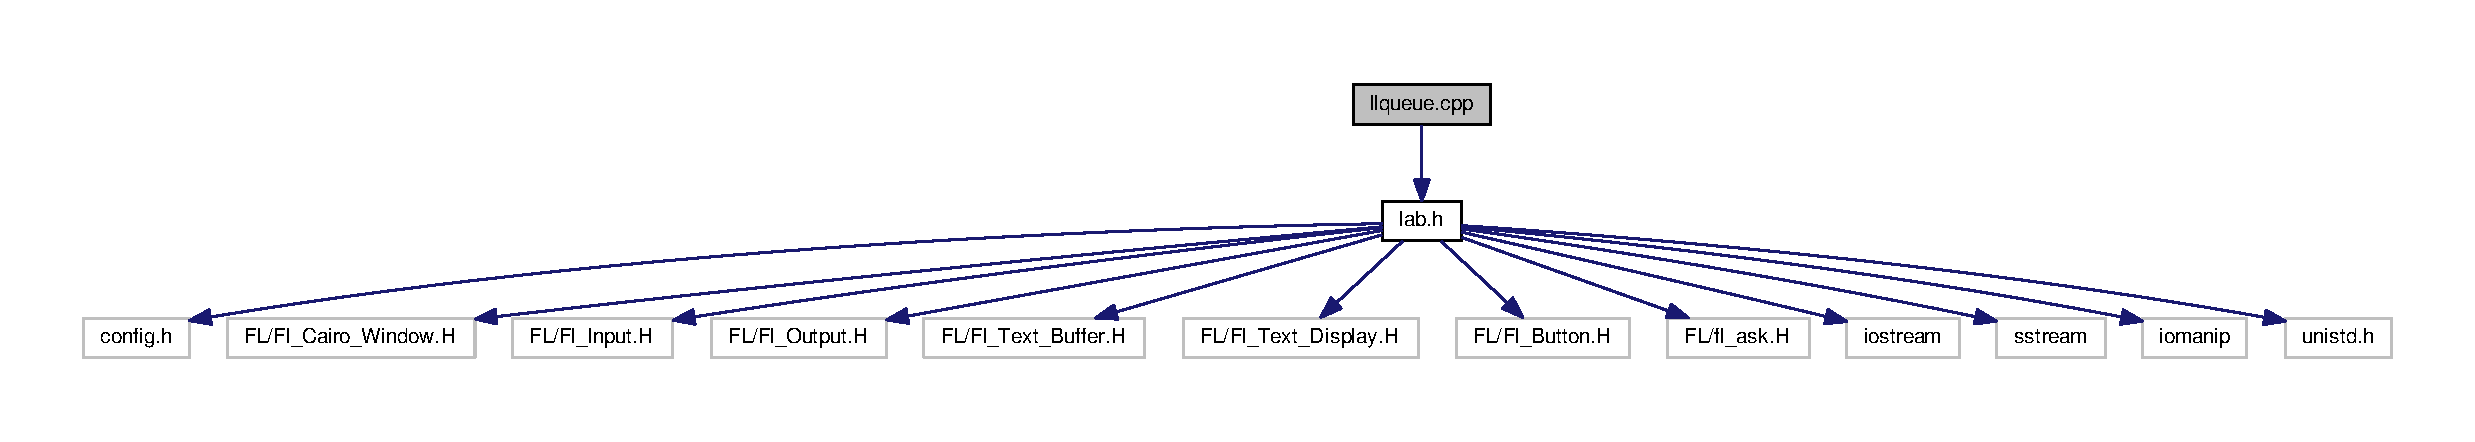
\includegraphics[width=350pt]{llqueue_8cpp__incl}
\end{center}
\end{figure}

\hypertarget{main_8cpp}{\subsection{main.\+cpp File Reference}
\label{main_8cpp}\index{main.\+cpp@{main.\+cpp}}
}
{\ttfamily \#include \char`\"{}lab.\+h\char`\"{}}\\*
Include dependency graph for main.\+cpp\+:\nopagebreak
\begin{figure}[H]
\begin{center}
\leavevmode
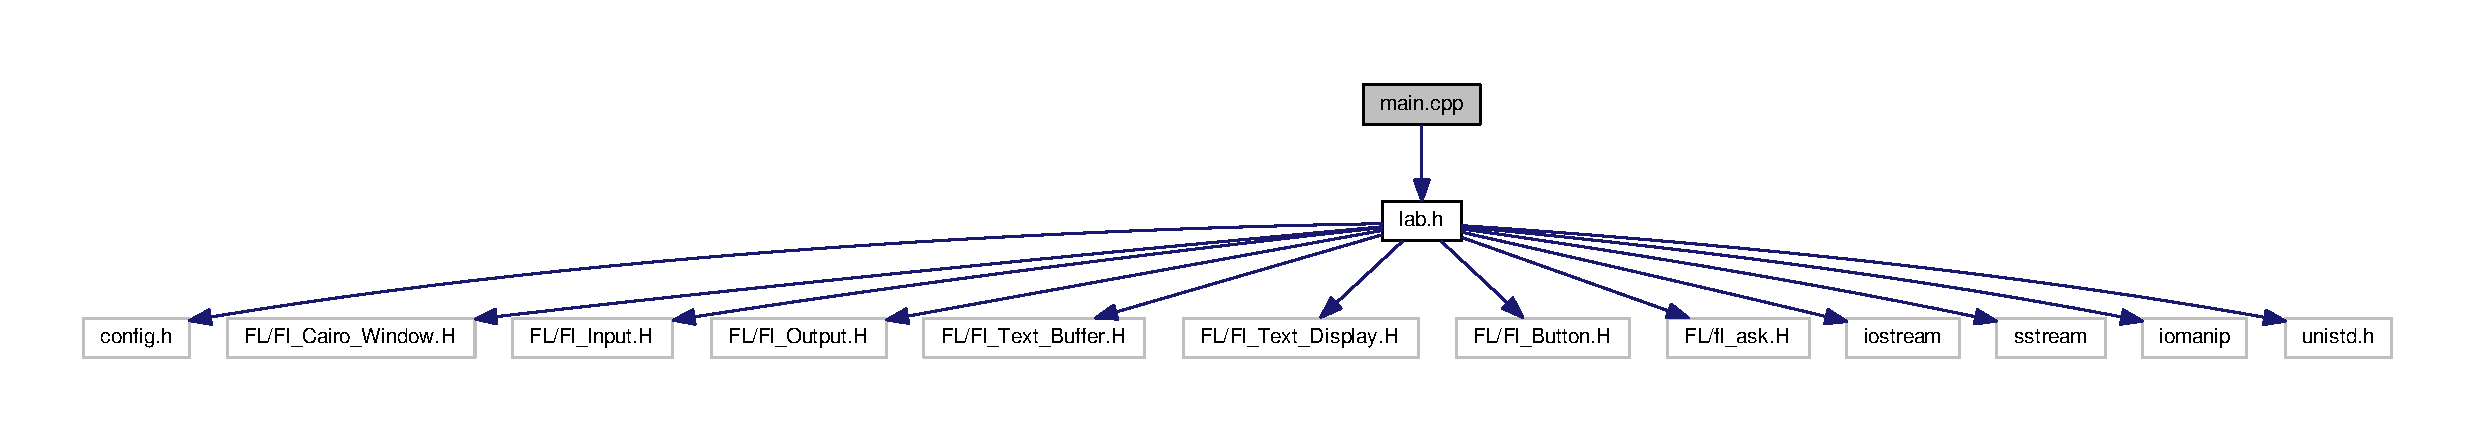
\includegraphics[width=350pt]{main_8cpp__incl}
\end{center}
\end{figure}
\subsubsection*{Functions}
\begin{DoxyCompactItemize}
\item 
int \hyperlink{main_8cpp_ae66f6b31b5ad750f1fe042a706a4e3d4}{main} ()
\end{DoxyCompactItemize}
\subsubsection*{Variables}
\begin{DoxyCompactItemize}
\item 
Fl\+\_\+\+Input $\ast$ \hyperlink{main_8cpp_abf805c82a90897837d1c26ef915f1cd6}{pizza}
\item 
Fl\+\_\+\+Input $\ast$ \hyperlink{main_8cpp_a0ce7586472726848924b4964b80e69ba}{address}
\item 
Fl\+\_\+\+Input $\ast$ \hyperlink{main_8cpp_a6f3dbb90a24ffb00549fdd15a79cbd66}{driver}
\item 
Fl\+\_\+\+Output $\ast$ \hyperlink{main_8cpp_a05c7f6e86cca5f4d0ebf44d1f5042c37}{watch}
\item 
Fl\+\_\+\+Text\+\_\+\+Buffer $\ast$ \hyperlink{main_8cpp_aea2b8efadc87a819fe57c311d668e504}{buff}
\item 
Fl\+\_\+\+Text\+\_\+\+Buffer $\ast$ \hyperlink{main_8cpp_a3a16cd8310a89f45962eb39b72bb9bb1}{cbuff}
\item 
Fl\+\_\+\+Text\+\_\+\+Buffer $\ast$ \hyperlink{main_8cpp_a5d487f4a7b5d36f823b8b1cb3db75aa4}{dbuff}
\item 
Fl\+\_\+\+Text\+\_\+\+Display $\ast$ \hyperlink{main_8cpp_a23f917547a833922fd6bc8797cc04ee1}{order\+Q}
\item 
Fl\+\_\+\+Text\+\_\+\+Display $\ast$ \hyperlink{main_8cpp_ad042fec17c471064617911f13dca15a8}{cooked\+Q}
\item 
Fl\+\_\+\+Text\+\_\+\+Display $\ast$ \hyperlink{main_8cpp_a20a356461cec27fe0d294f923f7ebd01}{driver\+Q}
\end{DoxyCompactItemize}


\subsubsection{Function Documentation}
\hypertarget{main_8cpp_ae66f6b31b5ad750f1fe042a706a4e3d4}{\index{main.\+cpp@{main.\+cpp}!main@{main}}
\index{main@{main}!main.\+cpp@{main.\+cpp}}
\paragraph[{main}]{\setlength{\rightskip}{0pt plus 5cm}int main (
\begin{DoxyParamCaption}
{}
\end{DoxyParamCaption}
)}}\label{main_8cpp_ae66f6b31b5ad750f1fe042a706a4e3d4}

\begin{DoxyCode}
18 \{
19     Fl\_Cairo\_Window cw(400,300); \textcolor{comment}{//width and height of the window}
20     cw.label(\textcolor{stringliteral}{"Pizza Deliveries"});\textcolor{comment}{//title of your window}
21     \textcolor{comment}{//cw.color(FL\_BLUE);}
22     
23     \hyperlink{main_8cpp_abf805c82a90897837d1c26ef915f1cd6}{pizza} = \textcolor{keyword}{new} Fl\_Input(180,20,100,20, \textcolor{stringliteral}{"Pizza:"});
24     \hyperlink{main_8cpp_abf805c82a90897837d1c26ef915f1cd6}{pizza}->labelcolor(FL\_BLUE);
25     
26     \hyperlink{main_8cpp_a0ce7586472726848924b4964b80e69ba}{address} = \textcolor{keyword}{new} Fl\_Input(180,40,100,20, \textcolor{stringliteral}{"Address:"});
27     \hyperlink{main_8cpp_a0ce7586472726848924b4964b80e69ba}{address}->labelcolor(FL\_BLUE);
28     
29     \hyperlink{main_8cpp_a6f3dbb90a24ffb00549fdd15a79cbd66}{driver} = \textcolor{keyword}{new} Fl\_Input(180,60,100,20, \textcolor{stringliteral}{"Driver:"});
30     \hyperlink{main_8cpp_a6f3dbb90a24ffb00549fdd15a79cbd66}{driver}->labelcolor(FL\_BLUE);
31     
32     \hyperlink{main_8cpp_a05c7f6e86cca5f4d0ebf44d1f5042c37}{watch} = \textcolor{keyword}{new} Fl\_Output(70,20,60,20, \textcolor{stringliteral}{"seconds:"});
33     
34     \hyperlink{main_8cpp_aea2b8efadc87a819fe57c311d668e504}{buff} = \textcolor{keyword}{new} Fl\_Text\_Buffer();
35     \hyperlink{main_8cpp_a23f917547a833922fd6bc8797cc04ee1}{orderQ} = \textcolor{keyword}{new} Fl\_Text\_Display(50,100,100,100,\textcolor{stringliteral}{"Order Q"});
36     \hyperlink{main_8cpp_a23f917547a833922fd6bc8797cc04ee1}{orderQ}->buffer(\hyperlink{main_8cpp_aea2b8efadc87a819fe57c311d668e504}{buff});
37     
38     \hyperlink{main_8cpp_a3a16cd8310a89f45962eb39b72bb9bb1}{cbuff} = \textcolor{keyword}{new} Fl\_Text\_Buffer();
39     \hyperlink{main_8cpp_ad042fec17c471064617911f13dca15a8}{cookedQ} = \textcolor{keyword}{new} Fl\_Text\_Display(150,100,100,100,\textcolor{stringliteral}{"Cooked Q"});
40     \hyperlink{main_8cpp_ad042fec17c471064617911f13dca15a8}{cookedQ}->buffer(\hyperlink{main_8cpp_a3a16cd8310a89f45962eb39b72bb9bb1}{cbuff});
41 
42     \hyperlink{main_8cpp_a5d487f4a7b5d36f823b8b1cb3db75aa4}{dbuff} = \textcolor{keyword}{new} Fl\_Text\_Buffer();
43     \hyperlink{main_8cpp_a20a356461cec27fe0d294f923f7ebd01}{driverQ} = \textcolor{keyword}{new} Fl\_Text\_Display(250,100,100,100,\textcolor{stringliteral}{"Driver Q"});
44     \hyperlink{main_8cpp_a20a356461cec27fe0d294f923f7ebd01}{driverQ}->buffer(\hyperlink{main_8cpp_a5d487f4a7b5d36f823b8b1cb3db75aa4}{dbuff});
45     
46     Fl\_Button b(280,35,50,20, \textcolor{stringliteral}{"Order"});
47     b.callback((Fl\_Callback*)\hyperlink{lab_8h_a547f84331a8c529348e1130ca169c69c}{order\_cb});
48     
49     Fl\_Button a(280,60,50,20, \textcolor{stringliteral}{"Add"});
50     a.callback((Fl\_Callback*)\hyperlink{driver__cb_8cpp_a2edcbf888225d725652a44b6a98d64c2}{driver\_cb});
51     cw.show();
52     Fl::add\_timeout(1,\hyperlink{lab_8h_a13ed8751dfa95731ad8930762493b16b}{timer});
53     \textcolor{keywordflow}{return} Fl::run();
54     \}
\end{DoxyCode}


\subsubsection{Variable Documentation}
\hypertarget{main_8cpp_a0ce7586472726848924b4964b80e69ba}{\index{main.\+cpp@{main.\+cpp}!address@{address}}
\index{address@{address}!main.\+cpp@{main.\+cpp}}
\paragraph[{address}]{\setlength{\rightskip}{0pt plus 5cm}Fl\+\_\+\+Input$\ast$ address}}\label{main_8cpp_a0ce7586472726848924b4964b80e69ba}
\hypertarget{main_8cpp_aea2b8efadc87a819fe57c311d668e504}{\index{main.\+cpp@{main.\+cpp}!buff@{buff}}
\index{buff@{buff}!main.\+cpp@{main.\+cpp}}
\paragraph[{buff}]{\setlength{\rightskip}{0pt plus 5cm}Fl\+\_\+\+Text\+\_\+\+Buffer$\ast$ buff}}\label{main_8cpp_aea2b8efadc87a819fe57c311d668e504}
\hypertarget{main_8cpp_a3a16cd8310a89f45962eb39b72bb9bb1}{\index{main.\+cpp@{main.\+cpp}!cbuff@{cbuff}}
\index{cbuff@{cbuff}!main.\+cpp@{main.\+cpp}}
\paragraph[{cbuff}]{\setlength{\rightskip}{0pt plus 5cm}Fl\+\_\+\+Text\+\_\+\+Buffer$\ast$ cbuff}}\label{main_8cpp_a3a16cd8310a89f45962eb39b72bb9bb1}
\hypertarget{main_8cpp_ad042fec17c471064617911f13dca15a8}{\index{main.\+cpp@{main.\+cpp}!cooked\+Q@{cooked\+Q}}
\index{cooked\+Q@{cooked\+Q}!main.\+cpp@{main.\+cpp}}
\paragraph[{cooked\+Q}]{\setlength{\rightskip}{0pt plus 5cm}Fl\+\_\+\+Text\+\_\+\+Display$\ast$ cooked\+Q}}\label{main_8cpp_ad042fec17c471064617911f13dca15a8}
\hypertarget{main_8cpp_a5d487f4a7b5d36f823b8b1cb3db75aa4}{\index{main.\+cpp@{main.\+cpp}!dbuff@{dbuff}}
\index{dbuff@{dbuff}!main.\+cpp@{main.\+cpp}}
\paragraph[{dbuff}]{\setlength{\rightskip}{0pt plus 5cm}Fl\+\_\+\+Text\+\_\+\+Buffer$\ast$ dbuff}}\label{main_8cpp_a5d487f4a7b5d36f823b8b1cb3db75aa4}
\hypertarget{main_8cpp_a6f3dbb90a24ffb00549fdd15a79cbd66}{\index{main.\+cpp@{main.\+cpp}!driver@{driver}}
\index{driver@{driver}!main.\+cpp@{main.\+cpp}}
\paragraph[{driver}]{\setlength{\rightskip}{0pt plus 5cm}Fl\+\_\+\+Input$\ast$ driver}}\label{main_8cpp_a6f3dbb90a24ffb00549fdd15a79cbd66}
\hypertarget{main_8cpp_a20a356461cec27fe0d294f923f7ebd01}{\index{main.\+cpp@{main.\+cpp}!driver\+Q@{driver\+Q}}
\index{driver\+Q@{driver\+Q}!main.\+cpp@{main.\+cpp}}
\paragraph[{driver\+Q}]{\setlength{\rightskip}{0pt plus 5cm}Fl\+\_\+\+Text\+\_\+\+Display$\ast$ driver\+Q}}\label{main_8cpp_a20a356461cec27fe0d294f923f7ebd01}
\hypertarget{main_8cpp_a23f917547a833922fd6bc8797cc04ee1}{\index{main.\+cpp@{main.\+cpp}!order\+Q@{order\+Q}}
\index{order\+Q@{order\+Q}!main.\+cpp@{main.\+cpp}}
\paragraph[{order\+Q}]{\setlength{\rightskip}{0pt plus 5cm}Fl\+\_\+\+Text\+\_\+\+Display$\ast$ order\+Q}}\label{main_8cpp_a23f917547a833922fd6bc8797cc04ee1}
\hypertarget{main_8cpp_abf805c82a90897837d1c26ef915f1cd6}{\index{main.\+cpp@{main.\+cpp}!pizza@{pizza}}
\index{pizza@{pizza}!main.\+cpp@{main.\+cpp}}
\paragraph[{pizza}]{\setlength{\rightskip}{0pt plus 5cm}Fl\+\_\+\+Input$\ast$ pizza}}\label{main_8cpp_abf805c82a90897837d1c26ef915f1cd6}
\hypertarget{main_8cpp_a05c7f6e86cca5f4d0ebf44d1f5042c37}{\index{main.\+cpp@{main.\+cpp}!watch@{watch}}
\index{watch@{watch}!main.\+cpp@{main.\+cpp}}
\paragraph[{watch}]{\setlength{\rightskip}{0pt plus 5cm}Fl\+\_\+\+Output$\ast$ watch}}\label{main_8cpp_a05c7f6e86cca5f4d0ebf44d1f5042c37}

\hypertarget{order__cb_8cpp}{\subsection{order\+\_\+cb.\+cpp File Reference}
\label{order__cb_8cpp}\index{order\+\_\+cb.\+cpp@{order\+\_\+cb.\+cpp}}
}
{\ttfamily \#include \char`\"{}lab.\+h\char`\"{}}\\*
Include dependency graph for order\+\_\+cb.\+cpp\+:\nopagebreak
\begin{figure}[H]
\begin{center}
\leavevmode
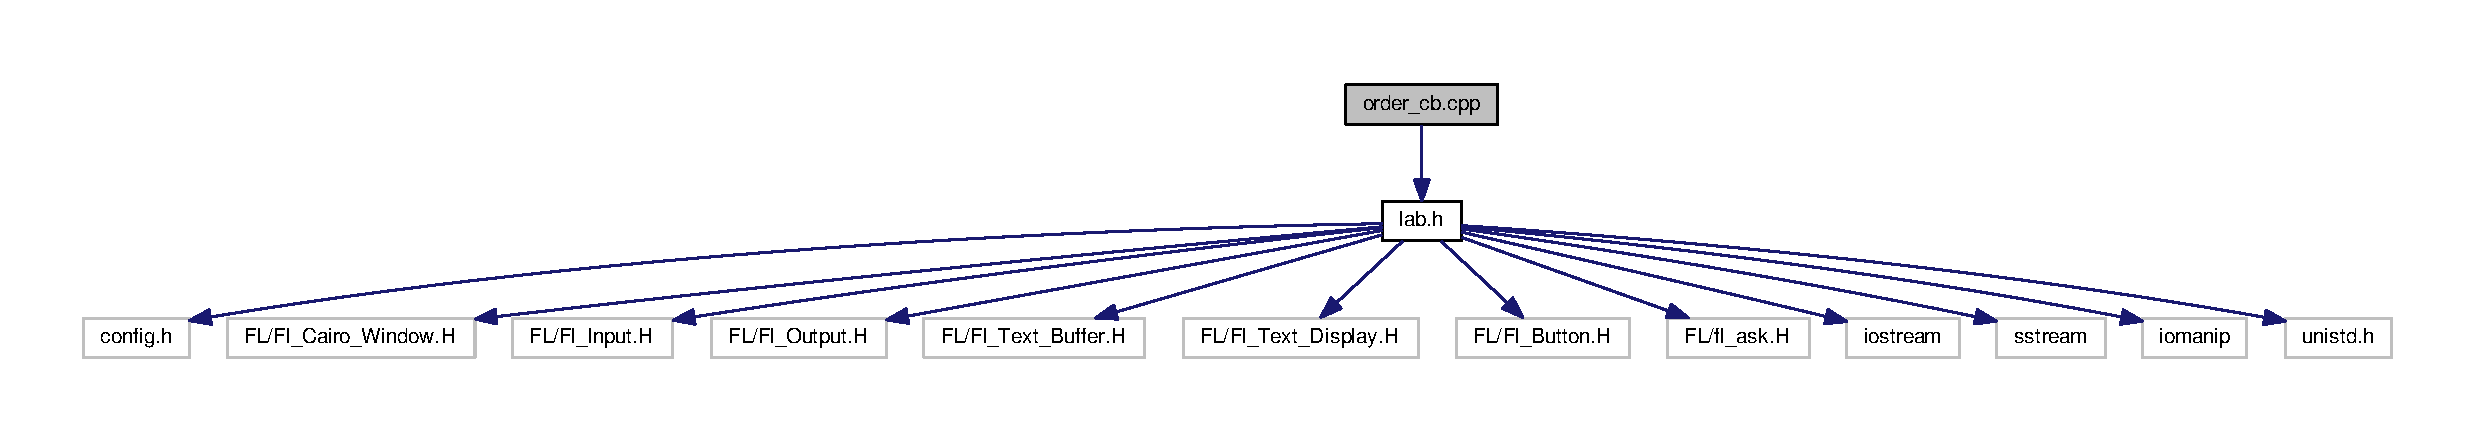
\includegraphics[width=350pt]{order__cb_8cpp__incl}
\end{center}
\end{figure}
\subsubsection*{Functions}
\begin{DoxyCompactItemize}
\item 
void \hyperlink{order__cb_8cpp_a547f84331a8c529348e1130ca169c69c}{order\+\_\+cb} (void $\ast$, void $\ast$)
\begin{DoxyCompactList}\small\item\em This is the callback function to order a pizza void pointers not used return void. \end{DoxyCompactList}\end{DoxyCompactItemize}
\subsubsection*{Variables}
\begin{DoxyCompactItemize}
\item 
\hyperlink{structORDER}{O\+R\+D\+E\+R} \hyperlink{order__cb_8cpp_a332f3283fc67e4d87244860ec1f0e880}{ord}
\item 
\hyperlink{classLLQUEUE}{L\+L\+Q\+U\+E\+U\+E} \hyperlink{order__cb_8cpp_a6131f0484df536b2c26a825ec37671a2}{o}
\item 
\hyperlink{classLLQUEUE}{L\+L\+Q\+U\+E\+U\+E} \hyperlink{order__cb_8cpp_a5574ed76bfb4e719e874d19f2d247625}{c}
\item 
\hyperlink{classRBQUEUE}{R\+B\+Q\+U\+E\+U\+E} \hyperlink{order__cb_8cpp_a87b7985f8561b2ac6c65961ab55b326e}{d}
\item 
\hyperlink{classRBQUEUE}{R\+B\+Q\+U\+E\+U\+E} \hyperlink{order__cb_8cpp_a0fc2dbd38da95932f1a2331561cf9a4e}{curr\+D}
\end{DoxyCompactItemize}


\subsubsection{Function Documentation}
\hypertarget{order__cb_8cpp_a547f84331a8c529348e1130ca169c69c}{\index{order\+\_\+cb.\+cpp@{order\+\_\+cb.\+cpp}!order\+\_\+cb@{order\+\_\+cb}}
\index{order\+\_\+cb@{order\+\_\+cb}!order\+\_\+cb.\+cpp@{order\+\_\+cb.\+cpp}}
\paragraph[{order\+\_\+cb}]{\setlength{\rightskip}{0pt plus 5cm}void order\+\_\+cb (
\begin{DoxyParamCaption}
\item[{void $\ast$}]{, }
\item[{void $\ast$}]{}
\end{DoxyParamCaption}
)}}\label{order__cb_8cpp_a547f84331a8c529348e1130ca169c69c}


This is the callback function to order a pizza void pointers not used return void. 


\begin{DoxyCode}
9 \{  
10     fl\_alert(\hyperlink{lab_8h_abf805c82a90897837d1c26ef915f1cd6}{pizza}->value()); \textcolor{comment}{//shows alert with input values}
11     fl\_alert(\hyperlink{lab_8h_a0ce7586472726848924b4964b80e69ba}{address}->value());
12    
13     \hyperlink{order__cb_8cpp_a332f3283fc67e4d87244860ec1f0e880}{ord}.\hyperlink{structORDER_aea87cd05ef2f7d3f6b2c5b9eebd0199d}{info} = \hyperlink{lab_8h_abf805c82a90897837d1c26ef915f1cd6}{pizza}->value(); 
14     \hyperlink{order__cb_8cpp_a332f3283fc67e4d87244860ec1f0e880}{ord}.\hyperlink{structORDER_a501ab180a46b15c372b77037ef5b3edc}{addr} = \hyperlink{lab_8h_a0ce7586472726848924b4964b80e69ba}{address}->value();
15    
16     \hyperlink{order__cb_8cpp_a6131f0484df536b2c26a825ec37671a2}{o}.\hyperlink{classLLQUEUE_a2d53817739f7c273a3c0f14f7804c065}{Insert}(\hyperlink{order__cb_8cpp_a332f3283fc67e4d87244860ec1f0e880}{ord});\textcolor{comment}{//inserts the data into order Q}
17     
18     \hyperlink{lab_8h_aea2b8efadc87a819fe57c311d668e504}{buff}->text((\hyperlink{order__cb_8cpp_a6131f0484df536b2c26a825ec37671a2}{o}.\hyperlink{classLLQUEUE_a0e9bffdcd903a132b8f7899ccdbc0315}{getQcontent}().c\_str())); \textcolor{comment}{// updates th order Q in FLTK}
19 
20     Fl::add\_timeout(10,\hyperlink{cook__cb_8cpp_abb6fd11336b6e04e134b70abc225a8f6}{cook\_cb}); \textcolor{comment}{//calls back the cook function }
21     \}
\end{DoxyCode}


\subsubsection{Variable Documentation}
\hypertarget{order__cb_8cpp_a5574ed76bfb4e719e874d19f2d247625}{\index{order\+\_\+cb.\+cpp@{order\+\_\+cb.\+cpp}!c@{c}}
\index{c@{c}!order\+\_\+cb.\+cpp@{order\+\_\+cb.\+cpp}}
\paragraph[{c}]{\setlength{\rightskip}{0pt plus 5cm}{\bf L\+L\+Q\+U\+E\+U\+E} c}}\label{order__cb_8cpp_a5574ed76bfb4e719e874d19f2d247625}
\hypertarget{order__cb_8cpp_a0fc2dbd38da95932f1a2331561cf9a4e}{\index{order\+\_\+cb.\+cpp@{order\+\_\+cb.\+cpp}!curr\+D@{curr\+D}}
\index{curr\+D@{curr\+D}!order\+\_\+cb.\+cpp@{order\+\_\+cb.\+cpp}}
\paragraph[{curr\+D}]{\setlength{\rightskip}{0pt plus 5cm}{\bf R\+B\+Q\+U\+E\+U\+E} curr\+D}}\label{order__cb_8cpp_a0fc2dbd38da95932f1a2331561cf9a4e}
\hypertarget{order__cb_8cpp_a87b7985f8561b2ac6c65961ab55b326e}{\index{order\+\_\+cb.\+cpp@{order\+\_\+cb.\+cpp}!d@{d}}
\index{d@{d}!order\+\_\+cb.\+cpp@{order\+\_\+cb.\+cpp}}
\paragraph[{d}]{\setlength{\rightskip}{0pt plus 5cm}{\bf R\+B\+Q\+U\+E\+U\+E} d}}\label{order__cb_8cpp_a87b7985f8561b2ac6c65961ab55b326e}
\hypertarget{order__cb_8cpp_a6131f0484df536b2c26a825ec37671a2}{\index{order\+\_\+cb.\+cpp@{order\+\_\+cb.\+cpp}!o@{o}}
\index{o@{o}!order\+\_\+cb.\+cpp@{order\+\_\+cb.\+cpp}}
\paragraph[{o}]{\setlength{\rightskip}{0pt plus 5cm}{\bf L\+L\+Q\+U\+E\+U\+E} o}}\label{order__cb_8cpp_a6131f0484df536b2c26a825ec37671a2}
\hypertarget{order__cb_8cpp_a332f3283fc67e4d87244860ec1f0e880}{\index{order\+\_\+cb.\+cpp@{order\+\_\+cb.\+cpp}!ord@{ord}}
\index{ord@{ord}!order\+\_\+cb.\+cpp@{order\+\_\+cb.\+cpp}}
\paragraph[{ord}]{\setlength{\rightskip}{0pt plus 5cm}{\bf O\+R\+D\+E\+R} ord}}\label{order__cb_8cpp_a332f3283fc67e4d87244860ec1f0e880}

\input{Remove_8cpp}
\hypertarget{remove_8cpp}{\subsection{remove.\+cpp File Reference}
\label{remove_8cpp}\index{remove.\+cpp@{remove.\+cpp}}
}
{\ttfamily \#include \char`\"{}lab.\+h\char`\"{}}\\*
Include dependency graph for remove.\+cpp\+:\nopagebreak
\begin{figure}[H]
\begin{center}
\leavevmode
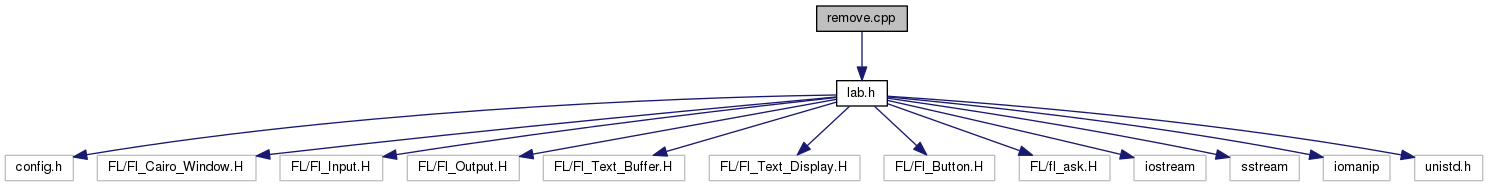
\includegraphics[width=350pt]{remove_8cpp__incl}
\end{center}
\end{figure}

\hypertarget{timer_8cpp}{\subsection{timer.\+cpp File Reference}
\label{timer_8cpp}\index{timer.\+cpp@{timer.\+cpp}}
}
{\ttfamily \#include \char`\"{}lab.\+h\char`\"{}}\\*
Include dependency graph for timer.\+cpp\+:\nopagebreak
\begin{figure}[H]
\begin{center}
\leavevmode
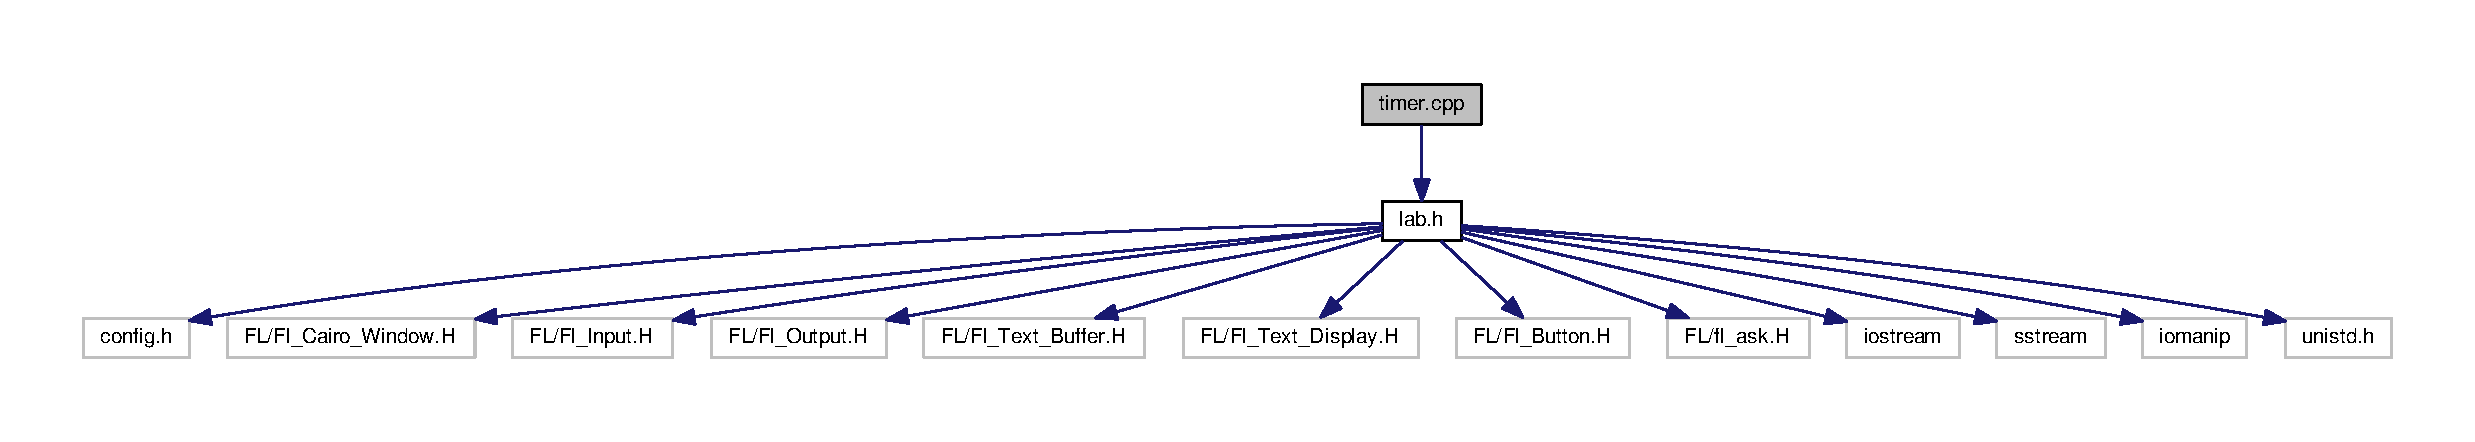
\includegraphics[width=350pt]{timer_8cpp__incl}
\end{center}
\end{figure}
\subsubsection*{Functions}
\begin{DoxyCompactItemize}
\item 
void \hyperlink{timer_8cpp_a13ed8751dfa95731ad8930762493b16b}{timer} (void $\ast$)
\begin{DoxyCompactList}\small\item\em This is a time function which keeps track of the time void pointers not used return void. \end{DoxyCompactList}\end{DoxyCompactItemize}


\subsubsection{Function Documentation}
\hypertarget{timer_8cpp_a13ed8751dfa95731ad8930762493b16b}{\index{timer.\+cpp@{timer.\+cpp}!timer@{timer}}
\index{timer@{timer}!timer.\+cpp@{timer.\+cpp}}
\paragraph[{timer}]{\setlength{\rightskip}{0pt plus 5cm}void timer (
\begin{DoxyParamCaption}
\item[{void $\ast$}]{}
\end{DoxyParamCaption}
)}}\label{timer_8cpp_a13ed8751dfa95731ad8930762493b16b}


This is a time function which keeps track of the time void pointers not used return void. 


\begin{DoxyCode}
4 \{
5     \textcolor{comment}{//std::cout << "1 sec" << std::endl;}
6     \textcolor{keyword}{static} \textcolor{keywordtype}{int} s = 0; \textcolor{keyword}{static} \textcolor{keywordtype}{int} m = 0;
7     std::ostringstream oss; 
8     
9     s++; \textcolor{keywordflow}{if} (s == 59) \{s=0; m++;\}
10     oss << std::setfill(\textcolor{charliteral}{'0'});
11     oss << std::setw(2) << m << \textcolor{stringliteral}{":"} << std::setw(2) << s;
12     \hyperlink{lab_8h_a05c7f6e86cca5f4d0ebf44d1f5042c37}{watch}->value(oss.str().c\_str());
13     
14     Fl::repeat\_timeout(1,\hyperlink{timer_8cpp_a13ed8751dfa95731ad8930762493b16b}{timer}); \textcolor{comment}{//repeats after every second}
15  
16 \}
\end{DoxyCode}

%--- End generated contents ---

% Index
\newpage
\phantomsection
\addcontentsline{toc}{section}{Index}
\printindex

\end{document}
